\section{Measurement Checks and Designs That Were Not Informative}\label{app:checks}

\subsection{Measurement checks on the age profile}

\paragraph{Child-years versus band means.} Table~\ref{tab:ige_sons} reports, next to the child-year regressions, a
version with one observation per child and the log of the band mean of at least two years, which averages out
transitory income within the band. The profile is the same: the White--Black gap in the family-income IGE is
$-0.005$ at 25--29, 0.154$^{***}$ at 30--34 and 0.191$^{***}$ at 35--39, and in the earnings IGE $-0.011$, 0.091$^{*}$
and 0.222$^{***}$.

\paragraph{Balanced panels.} In the panel of sons observed in every band of 25--49, the White--Black gap in the
family-income IGE is 0.007 at 25--29, 0.133 at 30--34, 0.189$^{**}$ at 35--39, 0.156$^{*}$ at 40--44 and 0.247$^{**}$
at 45--49, with a trend of 0.101$^{**}$ (0.046). A panel of sons observed in every band from 35 to 55 keeps only 351
Black and 745 White sons, selected on staying in the survey for two decades; its estimates are too imprecise to be
informative about later changes ($\chi^2(3)=2.32$, $p=0.510$).\footnote{\texttt{output/ige\_by\_age.md}, Sections 1b,
1c and 2. Code: \texttt{26.IGEByAge.py}.}

\paragraph{Single ages and growth of the same sons.} Figure~\ref{fig:ageprofile} shows the band estimates and the
Lee--Solon single-age curves for sons and daughters in the PSID and the NLSY79. Following the same sons from 25--29 to
35--39, family income grows with parental income by 0.216$^{***}$ for White and 0.121$^{***}$ for Black sons
(difference 0.096$^{*}$), and own earnings by a difference of 0.134$^{**}$; from 25--29 to 45--49 the earnings
difference is 0.284$^{***}$ (Table~\ref{tab:growth}).

\paragraph{Lifetime income and attrition.} Table~\ref{tab:lambda} reports the Haider--Solon coefficients of current on
lifetime income by age and race, and Table~\ref{tab:attrition} the probability of staying in the panel, and Table~\ref{tab:rankage} the rank
mobility statistics by age band.

\begin{figure}[!htbp]
\centering
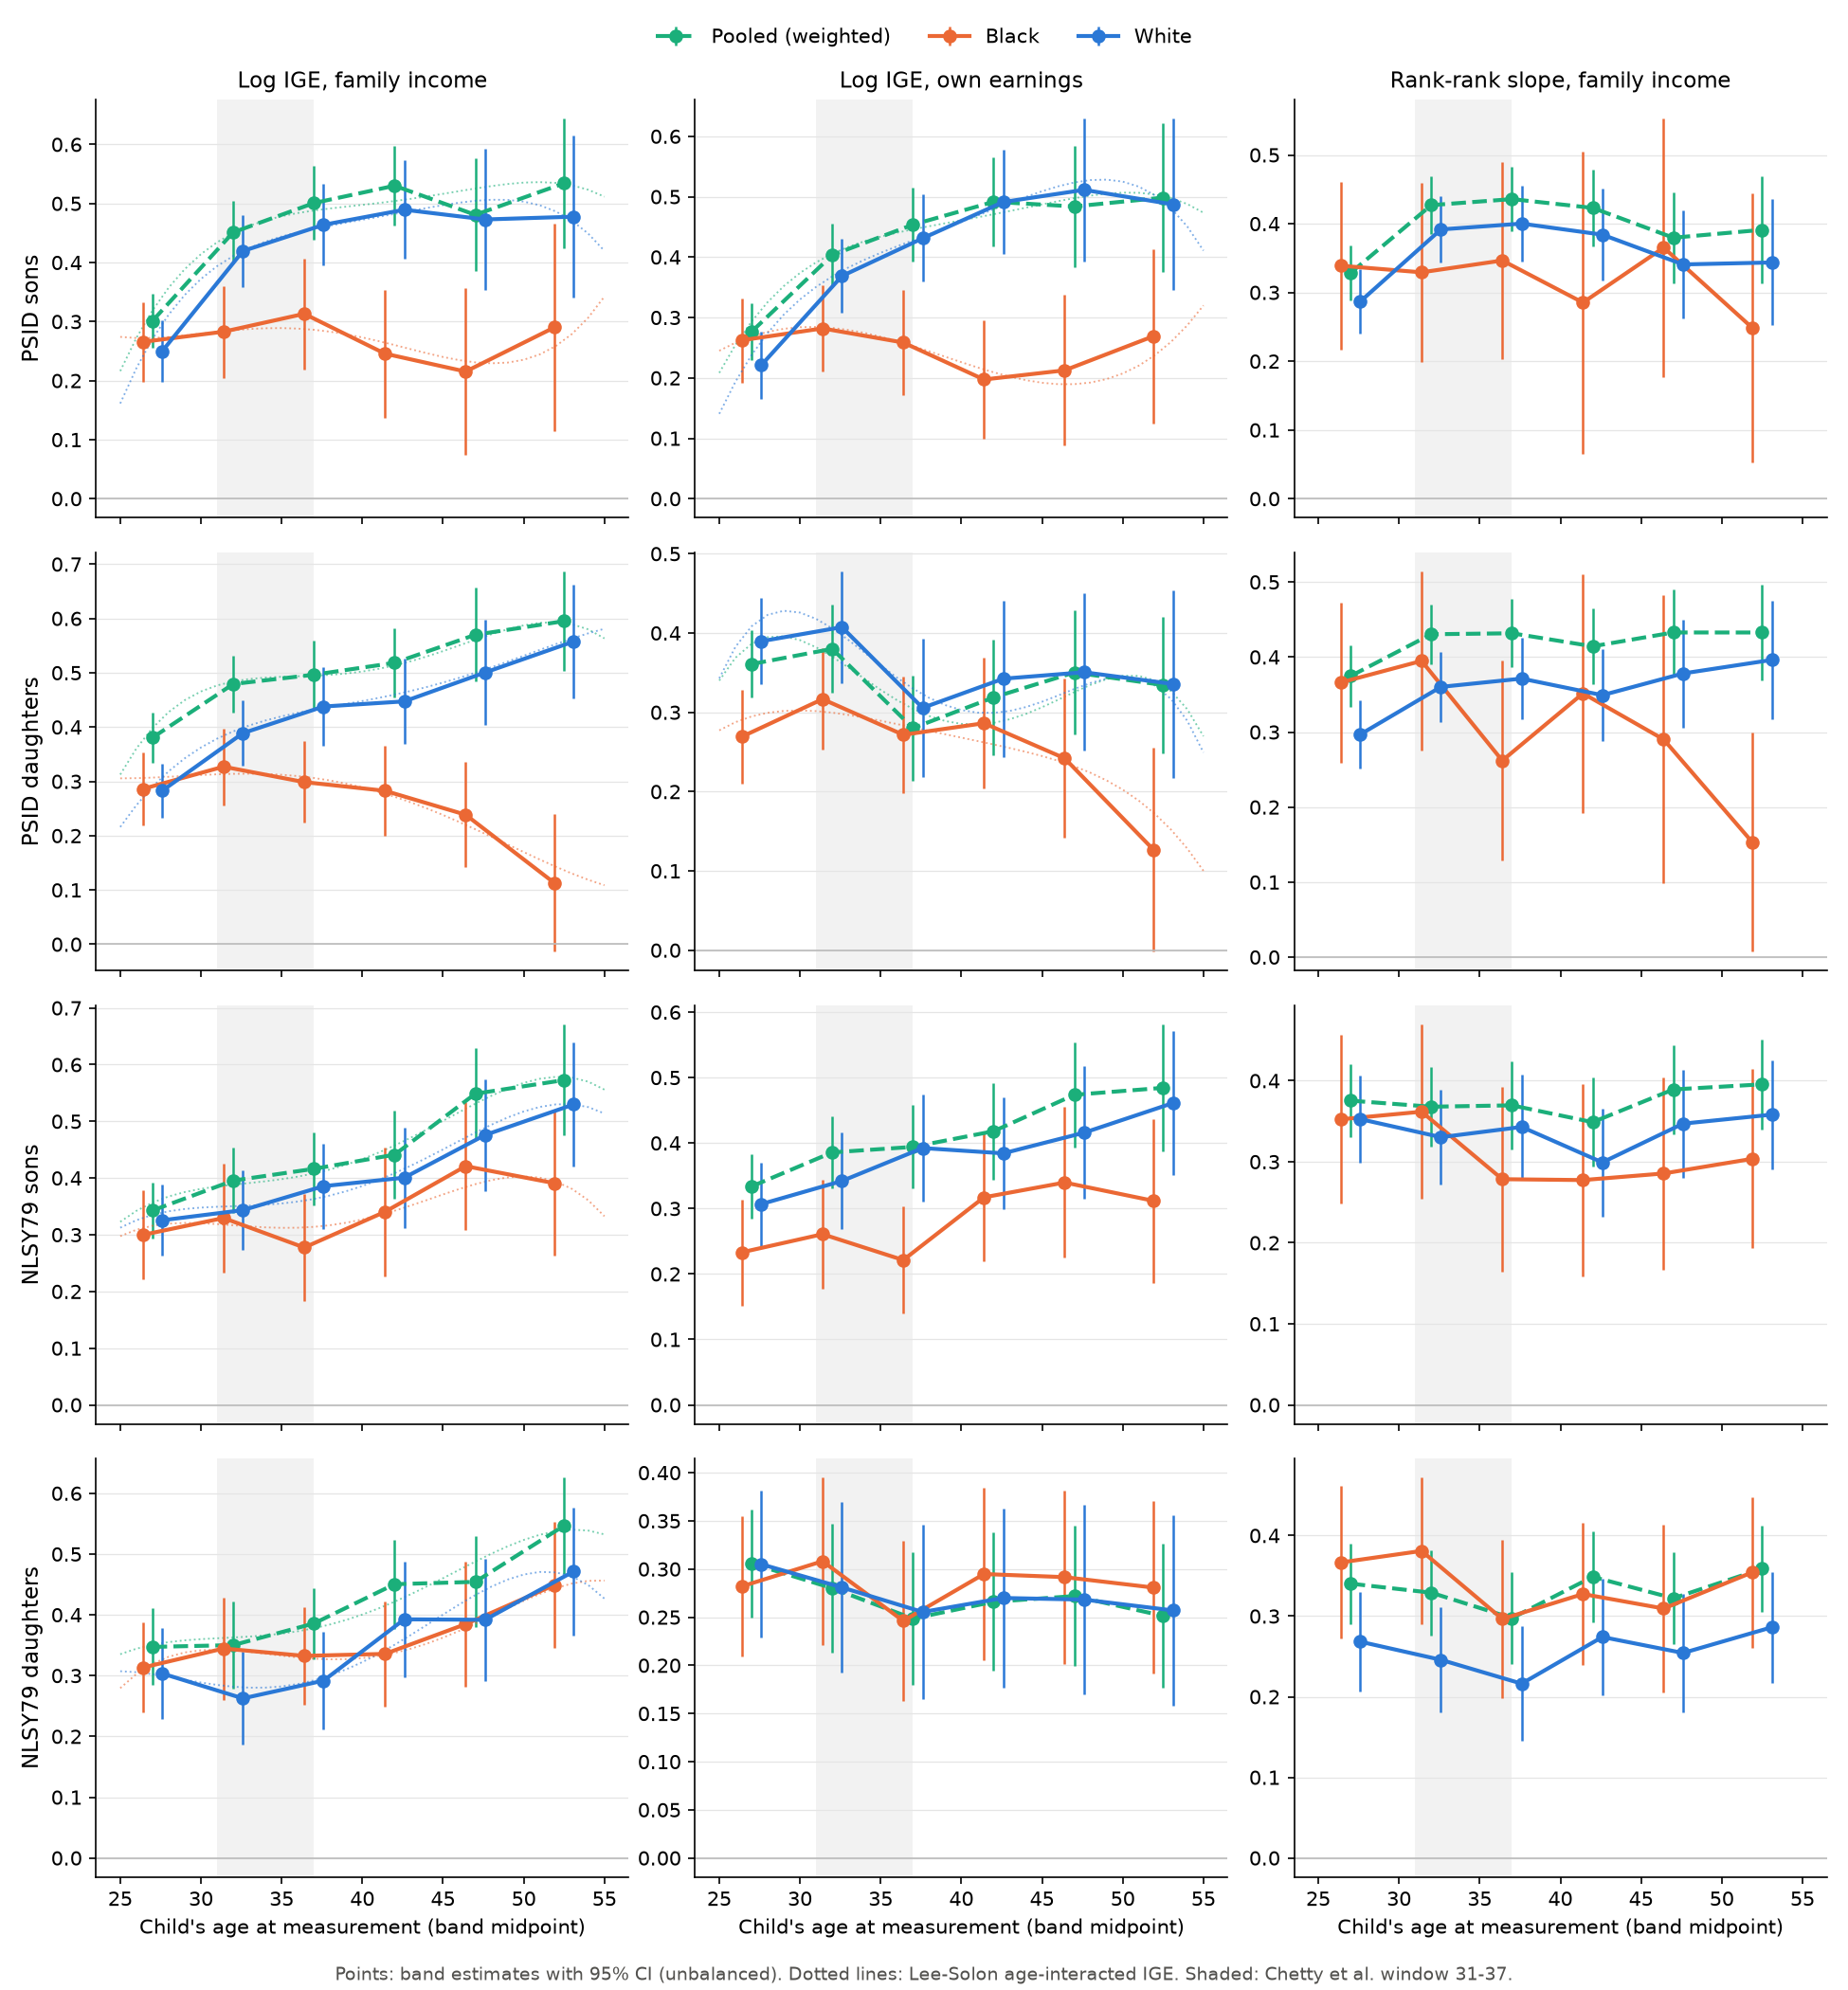
\includegraphics[width=\textwidth]{ige_by_age.png}
\caption{Intergenerational persistence by the child's age at measurement}\label{fig:ageprofile}
\begin{minipage}{\textwidth}\footnotesize \textit{Notes:} Points: band-specific estimates with 95\% confidence
intervals (unbalanced samples); dotted lines: Lee--Solon age-interacted IGE; shaded: the 31--37 window of
\citet{chetty2020race}. Columns: log IGE of family income, log IGE of own earnings, rank--rank slope of family income.
Rows: PSID sons, PSID daughters, NLSY79 sons, NLSY79 daughters. Code: \texttt{26.IGEByAge.py}.\end{minipage}
\end{figure}

\begin{table}[!htbp]
\centering
\caption{Log IGE of sons' income by age at measurement (PSID)}
\label{tab:ige_sons}
\resizebox{\ifdim\width>\textwidth\textwidth\else\width\fi}{!}{%
\resizebox*{!}{\ifdim\totalheight>0.85\textheight 0.85\textheight\else\totalheight\fi}{%
\begin{tabular}{lcc}
\toprule
Age band / group & \begin{tabular}[b]{@{}c@{}}ln own earnings\\(child-years)\end{tabular} & \begin{tabular}[b]{@{}c@{}}ln family income\\(child-years)\end{tabular} \\
 & (1) & (2) \\
\midrule
\multicolumn{3}{l}{\textit{Age 25--29}} \\
Pooled (weighted) & $0.276^{***}$ & $0.301^{***}$ \\
 & (0.024) & (0.023) \\
Black & $0.262^{***}$ & $0.266^{***}$ \\
 & (0.036) & (0.034) \\
White & $0.221^{***}$ & $0.250^{***}$ \\
 & (0.028) & (0.026) \\
White $-$ Black & $-0.041$ & $-0.016$ \\
 & (0.045) & (0.043) \\
Children (Black / White) & 1,607 / 2,474 & 1,662 / 2,506 \\
\addlinespace
\multicolumn{3}{l}{\textit{Age 30--34}} \\
Pooled (weighted) & $0.403^{***}$ & $0.451^{***}$ \\
 & (0.027) & (0.027) \\
Black & $0.282^{***}$ & $0.283^{***}$ \\
 & (0.037) & (0.040) \\
White & $0.369^{***}$ & $0.419^{***}$ \\
 & (0.031) & (0.031) \\
White $-$ Black & $0.087^{*}$ & $0.137^{***}$ \\
 & (0.048) & (0.050) \\
Children (Black / White) & 1,415 / 2,253 & 1,477 / 2,295 \\
\addlinespace
\multicolumn{3}{l}{\textit{Age 35--39}} \\
Pooled (weighted) & $0.454^{***}$ & $0.501^{***}$ \\
 & (0.031) & (0.032) \\
Black & $0.259^{***}$ & $0.313^{***}$ \\
 & (0.044) & (0.048) \\
White & $0.431^{***}$ & $0.464^{***}$ \\
 & (0.037) & (0.035) \\
White $-$ Black & $0.173^{***}$ & $0.151^{**}$ \\
 & (0.058) & (0.060) \\
Children (Black / White) & 1,068 / 1,838 & 1,125 / 1,884 \\
\addlinespace
\multicolumn{3}{l}{\textit{Age 40--44}} \\
Pooled (weighted) & $0.492^{***}$ & $0.530^{***}$ \\
 & (0.037) & (0.034) \\
Black & $0.197^{***}$ & $0.246^{***}$ \\
 & (0.050) & (0.055) \\
White & $0.491^{***}$ & $0.489^{***}$ \\
 & (0.044) & (0.043) \\
White $-$ Black & $0.294^{***}$ & $0.244^{***}$ \\
 & (0.067) & (0.070) \\
Children (Black / White) & 751 / 1,411 & 808 / 1,472 \\
\bottomrule
\end{tabular}}}
\par\smallskip
\begin{minipage}{\textwidth}\footnotesize \textit{Continued on the next table; notes below its last part.}\end{minipage}
\end{table}
\begin{table}[!htbp]
\centering
\addtocounter{table}{-1}
\caption{Log IGE of sons' income by age at measurement (PSID) (continued)}
\resizebox{\ifdim\width>\textwidth\textwidth\else\width\fi}{!}{%
\resizebox*{!}{\ifdim\totalheight>0.85\textheight 0.85\textheight\else\totalheight\fi}{%
\begin{tabular}{lcc}
\toprule
Age band / group & \begin{tabular}[b]{@{}c@{}}ln own earnings\\(child-years)\end{tabular} & \begin{tabular}[b]{@{}c@{}}ln family income\\(child-years)\end{tabular} \\
 & (1) & (2) \\
\midrule
\multicolumn{3}{l}{\textit{Age 45--49}} \\
Pooled (weighted) & $0.484^{***}$ & $0.481^{***}$ \\
 & (0.051) & (0.049) \\
Black & $0.213^{***}$ & $0.215^{***}$ \\
 & (0.064) & (0.072) \\
White & $0.511^{***}$ & $0.473^{***}$ \\
 & (0.060) & (0.061) \\
White $-$ Black & $0.299^{***}$ & $0.258^{***}$ \\
 & (0.088) & (0.095) \\
Children (Black / White) & 496 / 1,001 & 557 / 1,051 \\
\addlinespace
\multicolumn{3}{l}{\textit{Age 50--55}} \\
Pooled (weighted) & $0.498^{***}$ & $0.534^{***}$ \\
 & (0.063) & (0.056) \\
Black & $0.269^{***}$ & $0.290^{***}$ \\
 & (0.074) & (0.089) \\
White & $0.487^{***}$ & $0.478^{***}$ \\
 & (0.073) & (0.070) \\
White $-$ Black & $0.218^{**}$ & $0.187^{*}$ \\
 & (0.103) & (0.114) \\
Children (Black / White) & 351 / 726 & 420 / 780 \\
\addlinespace
\multicolumn{3}{l}{\textit{Age 31--37 (window of Chetty et al.)}} \\
Pooled (weighted) & $0.424^{***}$ & $0.475^{***}$ \\
 & (0.027) & (0.028) \\
Black & $0.292^{***}$ & $0.303^{***}$ \\
 & (0.036) & (0.041) \\
White & $0.392^{***}$ & $0.437^{***}$ \\
 & (0.032) & (0.031) \\
White $-$ Black & $0.099^{**}$ & $0.134^{***}$ \\
 & (0.048) & (0.051) \\
Children (Black / White) & 1,399 / 2,205 & 1,460 / 2,246 \\
\bottomrule
\end{tabular}}}
\par\smallskip
\begin{minipage}{\textwidth}\footnotesize \textit{Notes:} Each cell is the coefficient on log parental family income (mean over the child's ages 13--19) from a separate regression of the outcome in the column header, within the age band of the panel. Child-year columns: child-years in the band, controls for a quartic in the parent's age and single-year age dummies; band-mean columns (daughters' table; for sons in \texttt{output/ige\_by\_age.md}): one observation per child, log of the band mean ($\geq 2$ years), quartic in the parent's age and the mean age. Black and White: unweighted; Pooled: all races, weighted by the core longitudinal weight. White $-$ Black is the difference of the two race-specific regressions, estimated jointly. Standard errors clustered by 1968 family in parentheses. Race is the race of the parental household head. $^{***}$ $p<0.01$, $^{**}$ $p<0.05$, $^{*}$ $p<0.1$. Source: \texttt{26.IGEByAge.py} (\texttt{output/ige\_by\_age.csv}); table built by \texttt{28.PaperBTables.py}.\end{minipage}
\end{table}

\begin{table}[!htbp]
\centering
\caption{Who stays in the panel? Probability of being observed in a later age band (PSID)}
\label{tab:attrition}
\resizebox{\ifdim\width>\textwidth\textwidth\else\width\fi}{!}{%
\resizebox*{!}{\ifdim\totalheight>0.85\textheight 0.85\textheight\else\totalheight\fi}{%
\begin{tabular}{lcccc}
\toprule
 & \begin{tabular}[b]{@{}c@{}}30--34\end{tabular} & \begin{tabular}[b]{@{}c@{}}35--39\end{tabular} & \begin{tabular}[b]{@{}c@{}}40--44\end{tabular} & \begin{tabular}[b]{@{}c@{}}45--49\end{tabular} \\
 & (1) & (2) & (3) & (4) \\
\midrule
\multicolumn{5}{l}{\textit{Sons}} \\
Share observed, White & 0.903 & 0.799 & 0.696 & 0.584 \\
Share observed, Black & 0.809 & 0.640 & 0.521 & 0.403 \\
White: log parental income & $0.026^{**}$ & $0.068^{***}$ & $0.113^{***}$ & $0.139^{***}$ \\
 & (0.012) & (0.019) & (0.025) & (0.028) \\
Black: log parental income & $0.005$ & $-0.015$ & $-0.009$ & $0.005$ \\
 & (0.016) & (0.022) & (0.026) & (0.031) \\
White $-$ Black: log parental income & $0.021$ & $0.083^{***}$ & $0.122^{***}$ & $0.134^{***}$ \\
 & (0.020) & (0.029) & (0.036) & (0.041) \\
Children at risk & 3,767 & 3,385 & 2,912 & 2,453 \\
\addlinespace
\multicolumn{5}{l}{\textit{Daughters}} \\
Share observed, White & 0.923 & 0.835 & 0.737 & 0.612 \\
Share observed, Black & 0.886 & 0.791 & 0.703 & 0.581 \\
White: log parental income & $0.021^{**}$ & $0.031^{**}$ & $0.067^{***}$ & $0.122^{***}$ \\
 & (0.010) & (0.016) & (0.022) & (0.027) \\
Black: log parental income & $-0.009$ & $-0.016$ & $-0.031$ & $-0.012$ \\
 & (0.013) & (0.018) & (0.021) & (0.027) \\
White $-$ Black: log parental income & $0.030^{*}$ & $0.047^{**}$ & $0.098^{***}$ & $0.134^{***}$ \\
 & (0.016) & (0.024) & (0.030) & (0.038) \\
Children at risk & 4,330 & 3,851 & 3,315 & 2,764 \\
\bottomrule
\end{tabular}}}
\par\smallskip
\begin{minipage}{\textwidth}\footnotesize \textit{Notes:} Children with family income observed at 25--29 and born early enough to reach the band. Linear probability of being observed as a household head or spouse with valid family income in the band, on log parental income interacted with race, log family income at 25--29 interacted with race, a quartic in the parent's age and five-year birth-cohort dummies; standard errors clustered by 1968 family. $^{***}$ $p<0.01$, $^{**}$ $p<0.05$, $^{*}$ $p<0.1$. Source: \texttt{IGE/41.AgeProfileMeasurement.py} (\texttt{output/age\_profile\_measurement.csv}).\end{minipage}
\end{table}

\begin{table}[!htbp]
\centering
\caption{Current and lifetime income by age: Haider--Solon $\lambda$ by race (PSID, sons)}
\label{tab:lambda}
\resizebox{\ifdim\width>\textwidth\textwidth\else\width\fi}{!}{%
\resizebox*{!}{\ifdim\totalheight>0.85\textheight 0.85\textheight\else\totalheight\fi}{%
\begin{tabular}{lccccccc}
\toprule
 & \begin{tabular}[b]{@{}c@{}}25--29\end{tabular} & \begin{tabular}[b]{@{}c@{}}30--34\end{tabular} & \begin{tabular}[b]{@{}c@{}}35--39\end{tabular} & \begin{tabular}[b]{@{}c@{}}40--44\end{tabular} & \begin{tabular}[b]{@{}c@{}}45--49\end{tabular} & \begin{tabular}[b]{@{}c@{}}50--55\end{tabular} & \begin{tabular}[b]{@{}c@{}}Change, 35+\\minus below 35\end{tabular} \\
 & (1) & (2) & (3) & (4) & (5) & (6) & (7) \\
\midrule
\multicolumn{8}{l}{\textit{Own earnings}} \\
Black & $0.851^{***}$ & $0.999^{***}$ & $1.062^{***}$ & $1.123^{***}$ & $0.990^{***}$ & $1.022^{***}$ & $0.124^{*}$ \\
 & (0.076) & (0.050) & (0.060) & (0.074) & (0.055) & (0.093) & (0.072) \\
White & $0.688^{***}$ & $0.935^{***}$ & $1.051^{***}$ & $1.099^{***}$ & $1.216^{***}$ & $1.220^{***}$ & $0.335^{***}$ \\
 & (0.040) & (0.028) & (0.028) & (0.033) & (0.034) & (0.047) & (0.046) \\
White $-$ Black & $-0.163^{*}$ & $-0.064$ & $-0.011$ & $-0.024$ & $0.226^{***}$ & $0.198^{*}$ & $0.211^{**}$ \\
 & (0.086) & (0.057) & (0.066) & (0.081) & (0.065) & (0.105) & (0.086) \\
White $-$ Black, parental tercile 1 & $0.086$ & $-0.096$ & $-0.078$ & $-0.251^{**}$ & $0.361^{***}$ & $0.118$ & $0.043$ \\
 & (0.149) & (0.120) & (0.108) & (0.127) & (0.104) & (0.180) & (0.173) \\
White $-$ Black, parental tercile 2 & $-0.146$ & $-0.057$ & $-0.041$ & $0.182$ & $-0.041$ & $0.188$ & $0.173$ \\
 & (0.128) & (0.091) & (0.146) & (0.117) & (0.113) & (0.137) & (0.134) \\
White $-$ Black, parental tercile 3 & $-0.286^{**}$ & $0.124$ & $0.098$ & $0.289^{**}$ & $-0.174$ & $0.072$ & $0.153$ \\
 & (0.136) & (0.137) & (0.129) & (0.136) & (0.109) & (0.162) & (0.144) \\
Sons (Black / White) & 267 / 676 &  &  &  &  &  &  \\
\addlinespace
\multicolumn{8}{l}{\textit{Family income}} \\
Black & $0.817^{***}$ & $0.970^{***}$ & $1.052^{***}$ & $1.134^{***}$ & $1.096^{***}$ & $1.025^{***}$ & $0.183^{***}$ \\
 & (0.044) & (0.038) & (0.043) & (0.040) & (0.048) & (0.058) & (0.044) \\
White & $0.698^{***}$ & $0.894^{***}$ & $1.049^{***}$ & $1.067^{***}$ & $1.238^{***}$ & $1.280^{***}$ & $0.363^{***}$ \\
 & (0.030) & (0.027) & (0.027) & (0.026) & (0.033) & (0.040) & (0.037) \\
White $-$ Black & $-0.118^{**}$ & $-0.077$ & $-0.003$ & $-0.067$ & $0.142^{**}$ & $0.255^{***}$ & $0.179^{***}$ \\
 & (0.054) & (0.047) & (0.051) & (0.048) & (0.058) & (0.070) & (0.057) \\
White $-$ Black, parental tercile 1 & $0.105$ & $-0.135$ & $-0.102$ & $-0.185^{*}$ & $0.158$ & $0.264^{**}$ & $0.049$ \\
 & (0.104) & (0.129) & (0.090) & (0.095) & (0.108) & (0.107) & (0.133) \\
White $-$ Black, parental tercile 2 & $-0.106$ & $-0.088$ & $-0.006$ & $0.005$ & $0.013$ & $0.210^{*}$ & $0.153$ \\
 & (0.080) & (0.087) & (0.109) & (0.094) & (0.096) & (0.115) & (0.100) \\
White $-$ Black, parental tercile 3 & $-0.227^{**}$ & $0.009$ & $0.037$ & $0.195^{*}$ & $-0.050$ & $0.178$ & $0.199$ \\
 & (0.110) & (0.095) & (0.098) & (0.118) & (0.119) & (0.122) & (0.145) \\
Sons (Black / White) & 326 / 734 &  &  &  &  &  &  \\
\bottomrule
\end{tabular}}}
\par\smallskip
\begin{minipage}{\textwidth}\footnotesize \textit{Notes:} Sons with at least three valid years in each of 25--34, 35--44 and 45--55. $\lambda$: slope of the log outcome in the band (net of race-specific single-age means) on the son's mean of the same net log outcome over 25--55, by race, with single-age dummies; standard errors clustered by 1968 family. Adding log parental income to these regressions leaves $\lambda$ unchanged and its coefficient is not different from zero in any band (\texttt{output/age\_profile\_measurement.md}, Section C). $^{***}$ $p<0.01$, $^{**}$ $p<0.05$, $^{*}$ $p<0.1$. Source: \texttt{41.AgeProfileMeasurement.py} (\texttt{output/age\_profile\_measurement.csv}).\end{minipage}
\end{table}

\begin{table}[!htbp]
\centering
\caption{The racial gap in the log IGE by potential experience (PSID, sons)}
\label{tab:experience}
\resizebox{\ifdim\width>\textwidth\textwidth\else\width\fi}{!}{%
\resizebox*{!}{\ifdim\totalheight>0.85\textheight 0.85\textheight\else\totalheight\fi}{%
\begin{tabular}{lcccccc}
\toprule
 & \begin{tabular}[b]{@{}c@{}}0--4\end{tabular} & \begin{tabular}[b]{@{}c@{}}5--9\end{tabular} & \begin{tabular}[b]{@{}c@{}}10--14\end{tabular} & \begin{tabular}[b]{@{}c@{}}15--19\end{tabular} & \begin{tabular}[b]{@{}c@{}}20--24\end{tabular} & \begin{tabular}[b]{@{}c@{}}Opening\\($\geq$10 minus $<$10)\end{tabular} \\
 & (1) & (2) & (3) & (4) & (5) & (6) \\
\midrule
\multicolumn{7}{l}{\textit{Controls: single-year experience dummies}} \\
White $-$ Black gap, own earnings & $-0.121$ & $0.043$ & $0.118^{**}$ & $0.220^{***}$ & $0.272^{***}$ & $0.243^{***}$ \\
 & (0.101) & (0.044) & (0.051) & (0.059) & (0.066) & (0.067) \\
White $-$ Black gap, family income & $-0.100$ & $0.065$ & $0.168^{***}$ & $0.246^{***}$ & $0.216^{***}$ & $0.227^{***}$ \\
 & (0.093) & (0.044) & (0.052) & (0.060) & (0.071) & (0.065) \\
\addlinespace
\multicolumn{7}{l}{\textit{Controls: single-year age dummies}} \\
White $-$ Black gap, own earnings & $-0.123$ & $0.003$ & $0.059$ & $0.154^{***}$ & $0.196^{***}$ & $0.197^{***}$ \\
 & (0.099) & (0.043) & (0.046) & (0.055) & (0.063) & (0.064) \\
White $-$ Black gap, family income & $-0.099$ & $0.009$ & $0.094^{**}$ & $0.178^{***}$ & $0.143^{**}$ & $0.183^{***}$ \\
 & (0.092) & (0.043) & (0.047) & (0.056) & (0.067) & (0.062) \\
\bottomrule
\end{tabular}}}
\par\smallskip
\begin{minipage}{\textwidth}\footnotesize \textit{Notes:} Child-years at ages 20--55 as head or spouse, bands of potential experience (age $-$ completed years of schooling $-$ 6). Each cell: White $-$ Black difference of the band-specific log IGEs (stacked, clustered by 1968 family); controls: quartic in the parent's age and single-year age or experience dummies. At 25--29, sons of top-tercile White parents have 4.8 years of potential experience, other sons 6.0--7.0. $^{***}$ $p<0.01$, $^{**}$ $p<0.05$, $^{*}$ $p<0.1$. Source: \texttt{46.AgeProfileRound2.py} (\texttt{output/age\_profile\_round2.md}).\end{minipage}
\end{table}

\begin{table}[!htbp]
\centering
\caption{Schooling and ability: growth within cells and returns by age}
\label{tab:afqtgrowth}
\resizebox{\ifdim\width>\textwidth\textwidth\else\width\fi}{!}{%
\resizebox*{!}{\ifdim\totalheight>0.85\textheight 0.85\textheight\else\totalheight\fi}{%
\begin{tabular}{lccc}
\toprule
 & \begin{tabular}[b]{@{}c@{}}(1)\end{tabular} & \begin{tabular}[b]{@{}c@{}}(2)\end{tabular} & \begin{tabular}[b]{@{}c@{}}(3)\end{tabular} \\
 & (1) & (2) & (3) \\
\midrule
\multicolumn{4}{l}{\textit{PSID: same-employer wage growth at 25--34 on years of schooling}} \\
White & $0.010^{***}$ & $0.007^{***}$ & $0.009^{***}$ \\
 & (0.002) & (0.002) & (0.002) \\
Black & $0.003$ & $0.003$ & $0.001$ \\
 & (0.003) & (0.004) & (0.004) \\
White $-$ Black & $0.007^{**}$ & $0.004$ & $0.008$ \\
 & (0.003) & (0.005) & (0.005) \\
\addlinespace
\multicolumn{4}{l}{\textit{NLSY79: same-employer wage growth at 25--34 on years of schooling}} \\
White & $0.004^{***}$ & $0.004^{**}$ & $0.002$ \\
 & (0.001) & (0.001) & (0.001) \\
Black & $0.003$ & $-0.001$ & $-0.002$ \\
 & (0.002) & (0.002) & (0.003) \\
White $-$ Black & $0.002$ & $0.005^{*}$ & $0.004$ \\
 & (0.002) & (0.003) & (0.003) \\
\addlinespace
\multicolumn{4}{l}{\textit{NLSY79: log hourly rate of pay on AFQT (1 s.d.), by age}} \\
White: return to AFQT (1 s.d.) at 25--29 & $0.140^{***}$ &  & $0.103^{***}$ \\
 & (0.010) &  & (0.014) \\
White: rise of the return to AFQT (1 s.d.) & $0.110^{***}$ &  & $0.021^{*}$ \\
 & (0.010) &  & (0.013) \\
Black: return to AFQT (1 s.d.) at 25--29 & $0.188^{***}$ &  & $0.121^{***}$ \\
 & (0.017) &  & (0.020) \\
Black: rise of the return to AFQT (1 s.d.) & $0.098^{***}$ &  & $0.053^{**}$ \\
 & (0.019) &  & (0.022) \\
White $-$ Black: return to AFQT (1 s.d.) at 25--29 & $-0.048^{**}$ &  & $-0.018$ \\
 & (0.020) &  & (0.024) \\
White $-$ Black: rise of the return to AFQT (1 s.d.) & $0.012$ &  & $-0.031$ \\
 & (0.022) &  & (0.025) \\
\addlinespace
\multicolumn{4}{l}{\textit{NLSY79: log hourly rate of pay on years of schooling, by age}} \\
White: return to years of schooling at 25--29 &  & $0.048^{***}$ & $0.022^{***}$ \\
 &  & (0.004) & (0.005) \\
White: rise of the return to years of schooling &  & $0.057^{***}$ & $0.052^{***}$ \\
 &  & (0.004) & (0.005) \\
Black: return to years of schooling at 25--29 &  & $0.069^{***}$ & $0.043^{***}$ \\
 &  & (0.006) & (0.007) \\
Black: rise of the return to years of schooling &  & $0.042^{***}$ & $0.030^{***}$ \\
 &  & (0.006) & (0.007) \\
White $-$ Black: return to years of schooling at 25--29 &  & $-0.022^{***}$ & $-0.022^{**}$ \\
 &  & (0.007) & (0.008) \\
White $-$ Black: rise of the return to years of schooling &  & $0.015^{*}$ & $0.021^{**}$ \\
 &  & (0.008) & (0.009) \\
\bottomrule
\end{tabular}}}
\par\smallskip
\begin{minipage}{\textwidth}\footnotesize \textit{Notes:} Top panels: same-employer pairs at 25--34 (Table~\ref{tab:growthladder}); columns: (1) no cell controls, (2) fixed effects for the occupation group $\times$ industry group at the first interview of the pair, (3) for the early cell. Bottom panels: NLSY79 men 25--55, log hourly rate of pay on the AFQT (standardised within birth year) alone (1), schooling alone (2) or both (3), by age band; rise = mean over bands from 35 minus mean below 35. Employer learning predicts that with both included the schooling coefficient falls and the AFQT coefficient rises with experience. Controls: quartic in age, year (round) fixed effects. $^{***}$ $p<0.01$, $^{**}$ $p<0.05$, $^{*}$ $p<0.1$. Source: \texttt{45.WithinCellIdentification.py}.\end{minipage}
\end{table}

\begin{table}[!htbp]
\centering
\caption{Rank mobility of sons by age at measurement (PSID)}
\label{tab:rankage}
\resizebox{\ifdim\width>\textwidth\textwidth\else\width\fi}{!}{%
\resizebox*{!}{\ifdim\totalheight>0.85\textheight 0.85\textheight\else\totalheight\fi}{%
\begin{tabular}{lcccc}
\toprule
Age band / group & \begin{tabular}[b]{@{}c@{}}Rank--rank slope\\family income\end{tabular} & \begin{tabular}[b]{@{}c@{}}Expected rank\\at parental p25\end{tabular} & \begin{tabular}[b]{@{}c@{}}Expected rank\\at parental p75\end{tabular} & \begin{tabular}[b]{@{}c@{}}Rank--rank slope\\own earnings\end{tabular} \\
 & (1) & (2) & (3) & (4) \\
\midrule
\multicolumn{5}{l}{\textit{Age 25--29}} \\
Pooled (weighted) & $0.328^{***}$ & $40.7^{***}$ & $57.1^{***}$ & $0.300^{***}$ \\
 & (0.020) & (0.8) & (0.8) & (0.021) \\
Black & $0.339^{***}$ & $32.3^{***}$ & $49.2$ & $0.261^{***}$ \\
 & (0.062) & (1.3) & (3.5) & (0.067) \\
White & $0.287^{***}$ & $43.3^{***}$ & $57.6^{***}$ & $0.253^{***}$ \\
 & (0.024) & (1.0) & (0.8) & (0.023) \\
White $-$ Black & $-0.052$ & $11.0^{***}$ & $8.4^{**}$ & $-0.008$ \\
 & (0.067) & (1.6) & (3.6) & (0.071) \\
Children (Black / White) & 1,242 / 2,098 & 1,242 / 2,098 & 1,242 / 2,098 & 1,242 / 2,098 \\
\addlinespace
\multicolumn{5}{l}{\textit{Age 30--34}} \\
Pooled (weighted) & $0.427^{***}$ & $38.7^{***}$ & $60.1^{***}$ & $0.366^{***}$ \\
 & (0.022) & (0.9) & (0.8) & (0.020) \\
Black & $0.329^{***}$ & $31.3^{***}$ & $47.8$ & $0.299^{***}$ \\
 & (0.067) & (1.6) & (3.3) & (0.057) \\
White & $0.392^{***}$ & $41.1^{***}$ & $60.7^{***}$ & $0.322^{***}$ \\
 & (0.025) & (1.0) & (0.8) & (0.023) \\
White $-$ Black & $0.062$ & $9.8^{***}$ & $12.9^{***}$ & $0.024$ \\
 & (0.071) & (1.9) & (3.4) & (0.061) \\
Children (Black / White) & 1,141 / 1,932 & 1,141 / 1,932 & 1,141 / 1,932 & 1,141 / 1,932 \\
\addlinespace
\multicolumn{5}{l}{\textit{Age 35--39}} \\
Pooled (weighted) & $0.436^{***}$ & $38.9^{***}$ & $60.7^{***}$ & $0.356^{***}$ \\
 & (0.024) & (0.9) & (0.8) & (0.021) \\
Black & $0.346^{***}$ & $32.3^{***}$ & $49.6$ & $0.279^{***}$ \\
 & (0.073) & (1.5) & (3.9) & (0.065) \\
White & $0.400^{***}$ & $41.0^{***}$ & $61.0^{***}$ & $0.325^{***}$ \\
 & (0.028) & (1.2) & (0.9) & (0.025) \\
White $-$ Black & $0.054$ & $8.7^{***}$ & $11.4^{***}$ & $0.046$ \\
 & (0.079) & (1.9) & (4.0) & (0.069) \\
Children (Black / White) & 875 / 1,569 & 875 / 1,569 & 875 / 1,569 & 875 / 1,569 \\
\addlinespace
\multicolumn{5}{l}{\textit{Age 40--44}} \\
Pooled (weighted) & $0.423^{***}$ & $38.7^{***}$ & $59.8^{***}$ & $0.368^{***}$ \\
 & (0.028) & (1.2) & (1.0) & (0.027) \\
Black & $0.285^{**}$ & $32.7^{***}$ & $47.0$ & $0.202^{***}$ \\
 & (0.112) & (1.9) & (6.6) & (0.077) \\
White & $0.384^{***}$ & $40.7^{***}$ & $59.9^{***}$ & $0.352^{***}$ \\
 & (0.034) & (1.5) & (1.0) & (0.032) \\
White $-$ Black & $0.099$ & $8.0^{***}$ & $12.9^{*}$ & $0.150^{*}$ \\
 & (0.117) & (2.4) & (6.7) & (0.083) \\
Children (Black / White) & 572 / 1,175 & 572 / 1,175 & 572 / 1,175 & 572 / 1,175 \\
\bottomrule
\end{tabular}}}
\par\smallskip
\begin{minipage}{\textwidth}\footnotesize \textit{Continued on the next table; notes below its last part.}\end{minipage}
\end{table}
\begin{table}[!htbp]
\centering
\addtocounter{table}{-1}
\caption{Rank mobility of sons by age at measurement (PSID) (continued)}
\resizebox{\ifdim\width>\textwidth\textwidth\else\width\fi}{!}{%
\resizebox*{!}{\ifdim\totalheight>0.85\textheight 0.85\textheight\else\totalheight\fi}{%
\begin{tabular}{lcccc}
\toprule
Age band / group & \begin{tabular}[b]{@{}c@{}}Rank--rank slope\\family income\end{tabular} & \begin{tabular}[b]{@{}c@{}}Expected rank\\at parental p25\end{tabular} & \begin{tabular}[b]{@{}c@{}}Expected rank\\at parental p75\end{tabular} & \begin{tabular}[b]{@{}c@{}}Rank--rank slope\\own earnings\end{tabular} \\
 & (1) & (2) & (3) & (4) \\
\midrule
\multicolumn{5}{l}{\textit{Age 45--49}} \\
Pooled (weighted) & $0.380^{***}$ & $40.4^{***}$ & $59.3^{***}$ & $0.336^{***}$ \\
 & (0.034) & (1.4) & (1.2) & (0.034) \\
Black & $0.365^{***}$ & $34.4^{***}$ & $52.7$ & $0.258^{***}$ \\
 & (0.096) & (2.6) & (5.5) & (0.098) \\
White & $0.341^{***}$ & $42.4^{***}$ & $59.4^{***}$ & $0.314^{***}$ \\
 & (0.040) & (1.7) & (1.2) & (0.039) \\
White $-$ Black & $-0.024$ & $8.0^{**}$ & $6.7$ & $0.056$ \\
 & (0.104) & (3.1) & (5.7) & (0.106) \\
Children (Black / White) & 405 / 821 & 405 / 821 & 405 / 821 & 405 / 821 \\
\addlinespace
\multicolumn{5}{l}{\textit{Age 50--55}} \\
Pooled (weighted) & $0.391^{***}$ & $40.5^{***}$ & $60.0^{***}$ & $0.350^{***}$ \\
 & (0.040) & (1.6) & (1.4) & (0.041) \\
Black & $0.248^{**}$ & $32.0^{***}$ & $44.4$ & $0.213^{*}$ \\
 & (0.100) & (2.0) & (5.4) & (0.113) \\
White & $0.344^{***}$ & $42.8^{***}$ & $60.0^{***}$ & $0.317^{***}$ \\
 & (0.047) & (1.9) & (1.5) & (0.048) \\
White $-$ Black & $0.095$ & $10.8^{***}$ & $15.6^{***}$ & $0.104$ \\
 & (0.110) & (2.8) & (5.6) & (0.123) \\
Children (Black / White) & 339 / 613 & 339 / 613 & 339 / 613 & 339 / 613 \\
\addlinespace
\multicolumn{5}{l}{\textit{Age 31--37 (window of Chetty et al.)}} \\
Pooled (weighted) & $0.442^{***}$ & $38.7^{***}$ & $60.8^{***}$ & $0.372^{***}$ \\
 & (0.022) & (0.9) & (0.8) & (0.020) \\
Black & $0.348^{***}$ & $30.3^{***}$ & $47.7$ & $0.308^{***}$ \\
 & (0.064) & (1.5) & (3.2) & (0.061) \\
White & $0.397^{***}$ & $41.5^{***}$ & $61.3^{***}$ & $0.324^{***}$ \\
 & (0.025) & (1.0) & (0.8) & (0.022) \\
White $-$ Black & $0.048$ & $11.2^{***}$ & $13.6^{***}$ & $0.017$ \\
 & (0.069) & (1.8) & (3.3) & (0.065) \\
Children (Black / White) & 1,179 / 1,924 & 1,179 / 1,924 & 1,179 / 1,924 & 1,179 / 1,924 \\
\addlinespace
\multicolumn{5}{l}{\textit{Tests on the White $-$ Black slope gap across bands 25--29 to 50--55}} \\
Equal in all bands: Wald $\chi^2$ [p-value] & $\chi^2(5)=5.17$ &  &  & $\chi^2(5)=4.13$ \\
 & [0.396] &  &  & [0.530] \\
Linear trend per 10 years of age & $0.030$ &  &  & $0.043$ \\
 & (0.044) &  &  & (0.047) \\
\bottomrule
\end{tabular}}}
\par\smallskip
\begin{minipage}{\textwidth}\footnotesize \textit{Notes:} Child's band-mean family income (columns 1--3) or own earnings (column 4, zeros kept) ranked within birth year and band; parents' family income (mean at the child's ages 12--17) ranked within the child's birth year. Columns (2) and (3) evaluate the rank--rank line of column (1) at the 25th and 75th parental percentiles. All rank statistics weighted (core longitudinal weight at 16). Standard errors clustered by 1968 family in parentheses. $^{***}$ $p<0.01$, $^{**}$ $p<0.05$, $^{*}$ $p<0.1$. Source: \texttt{26.IGEByAge.py} (\texttt{output/ige\_by\_age.csv}); table built by \texttt{28.PaperBTables.py}.\end{minipage}
\end{table}

\begin{table}[!htbp]
\centering
\caption{Income growth by parental income: the same sons observed early and late (PSID)}
\label{tab:growth}
\resizebox{\ifdim\width>\textwidth\textwidth\else\width\fi}{!}{%
\resizebox*{!}{\ifdim\totalheight>0.85\textheight 0.85\textheight\else\totalheight\fi}{%
\begin{tabular}{lcccccc}
\toprule
Panel / group & \begin{tabular}[b]{@{}c@{}}ln family income\\early band\end{tabular} & \begin{tabular}[b]{@{}c@{}}ln family income\\late band\end{tabular} & \begin{tabular}[b]{@{}c@{}}Growth\\(late $-$ early)\end{tabular} & \begin{tabular}[b]{@{}c@{}}ln own earnings\\early band\end{tabular} & \begin{tabular}[b]{@{}c@{}}ln own earnings\\late band\end{tabular} & \begin{tabular}[b]{@{}c@{}}Growth\\(late $-$ early)\end{tabular} \\
 & (1) & (2) & (3) & (4) & (5) & (6) \\
\midrule
\multicolumn{7}{l}{\textit{Early band 25--29, late band 35--39}} \\
Pooled (weighted) & $0.310^{***}$ & $0.519^{***}$ & $0.210^{***}$ & $0.265^{***}$ & $0.465^{***}$ & $0.200^{***}$ \\
 & (0.028) & (0.034) & (0.031) & (0.029) & (0.035) & (0.035) \\
Black & $0.250^{***}$ & $0.376^{***}$ & $0.121^{***}$ & $0.262^{***}$ & $0.348^{***}$ & $0.085^{*}$ \\
 & (0.045) & (0.052) & (0.045) & (0.047) & (0.052) & (0.044) \\
White & $0.258^{***}$ & $0.473^{***}$ & $0.216^{***}$ & $0.211^{***}$ & $0.430^{***}$ & $0.219^{***}$ \\
 & (0.031) & (0.035) & (0.031) & (0.034) & (0.037) & (0.038) \\
White $-$ Black & $0.008$ & $0.097$ & $0.096^{*}$ & $-0.051$ & $0.081$ & $0.134^{**}$ \\
 & (0.055) & (0.063) & (0.055) & (0.058) & (0.064) & (0.058) \\
Children (Black / White) & 893 / 1,713 & 893 / 1,713 & 893 / 1,713 & 840 / 1,666 & 840 / 1,666 & 840 / 1,666 \\
\addlinespace
\multicolumn{7}{l}{\textit{Early band 25--29, late band 45--49}} \\
Pooled (weighted) & $0.337^{***}$ & $0.475^{***}$ & $0.146^{***}$ & $0.266^{***}$ & $0.477^{***}$ & $0.213^{***}$ \\
 & (0.038) & (0.052) & (0.047) & (0.040) & (0.064) & (0.055) \\
Black & $0.219^{***}$ & $0.189^{**}$ & $-0.030$ & $0.178^{***}$ & $0.166^{*}$ & $-0.011$ \\
 & (0.061) & (0.091) & (0.073) & (0.061) & (0.088) & (0.061) \\
White & $0.294^{***}$ & $0.464^{***}$ & $0.182^{***}$ & $0.245^{***}$ & $0.515^{***}$ & $0.273^{***}$ \\
 & (0.043) & (0.064) & (0.053) & (0.046) & (0.073) & (0.060) \\
White $-$ Black & $0.075$ & $0.275^{**}$ & $0.212^{**}$ & $0.067$ & $0.349^{***}$ & $0.284^{***}$ \\
 & (0.075) & (0.111) & (0.090) & (0.076) & (0.114) & (0.086) \\
Children (Black / White) & 423 / 938 & 423 / 938 & 423 / 938 & 371 / 896 & 371 / 896 & 371 / 896 \\
\addlinespace
\multicolumn{7}{l}{\textit{Early band 30--34, late band 40--44}} \\
Pooled (weighted) & $0.471^{***}$ & $0.491^{***}$ & $0.021$ & $0.431^{***}$ & $0.480^{***}$ & $0.050$ \\
 & (0.041) & (0.039) & (0.036) & (0.041) & (0.044) & (0.039) \\
Black & $0.271^{***}$ & $0.273^{***}$ & $0.003$ & $0.238^{***}$ & $0.253^{***}$ & $0.020$ \\
 & (0.061) & (0.059) & (0.064) & (0.055) & (0.058) & (0.049) \\
White & $0.445^{***}$ & $0.473^{***}$ & $0.027$ & $0.399^{***}$ & $0.465^{***}$ & $0.066^{*}$ \\
 & (0.040) & (0.045) & (0.036) & (0.041) & (0.045) & (0.036) \\
White $-$ Black & $0.174^{**}$ & $0.200^{***}$ & $0.025$ & $0.161^{**}$ & $0.212^{***}$ & $0.045$ \\
 & (0.073) & (0.074) & (0.073) & (0.069) & (0.073) & (0.060) \\
Children (Black / White) & 703 / 1,398 & 703 / 1,398 & 703 / 1,398 & 644 / 1,335 & 644 / 1,335 & 644 / 1,335 \\
\bottomrule
\end{tabular}}}
\par\smallskip
\begin{minipage}{\textwidth}\footnotesize \textit{Notes:} One observation per son observed in both bands of the panel. Columns (1), (2), (4), (5): the band-mean outcome on log parental income; columns (3) and (6): the change in the band-mean outcome on log parental income (controls: quartic in the parent's age and the change in mean age). A positive growth coefficient means that sons of richer parents have steeper income growth between the two bands, which raises the IGE measured later in life \citep{haider2006life}. Standard errors clustered by 1968 family. $^{***}$ $p<0.01$, $^{**}$ $p<0.05$, $^{*}$ $p<0.1$. Source: \texttt{IGE/26.IGEByAge.py} (\texttt{output/ige\_by\_age.csv}); table built by \texttt{IGE/28.PaperBTables.py}.\end{minipage}
\end{table}

\begin{table}[!htbp]
\centering
\caption{Log IGE of daughters' income by age at measurement (PSID)}
\label{tab:ige_daughters}
\resizebox{\ifdim\width>\textwidth\textwidth\else\width\fi}{!}{%
\resizebox*{!}{\ifdim\totalheight>0.85\textheight 0.85\textheight\else\totalheight\fi}{%
\begin{tabular}{lcccc}
\toprule
Age band / group & \begin{tabular}[b]{@{}c@{}}ln own earnings\\(child-years)\end{tabular} & \begin{tabular}[b]{@{}c@{}}ln family income\\(child-years)\end{tabular} & \begin{tabular}[b]{@{}c@{}}ln own earnings\\(band mean)\end{tabular} & \begin{tabular}[b]{@{}c@{}}ln family income\\(band mean)\end{tabular} \\
 & (1) & (2) & (3) & (4) \\
\midrule
\multicolumn{5}{l}{\textit{Age 25--29}} \\
Pooled (weighted) & $0.361^{***}$ & $0.381^{***}$ & $0.346^{***}$ & $0.359^{***}$ \\
 & (0.022) & (0.023) & (0.022) & (0.022) \\
Black & $0.269^{***}$ & $0.286^{***}$ & $0.263^{***}$ & $0.291^{***}$ \\
 & (0.030) & (0.034) & (0.031) & (0.031) \\
White & $0.390^{***}$ & $0.283^{***}$ & $0.375^{***}$ & $0.274^{***}$ \\
 & (0.028) & (0.025) & (0.026) & (0.025) \\
White $-$ Black & $0.120^{***}$ & $-0.003$ & $0.112^{***}$ & $-0.017$ \\
 & (0.041) & (0.042) & (0.040) & (0.039) \\
Children (Black / White) & 1,888 / 2,540 & 2,085 / 2,702 & 1,502 / 2,176 & 1,812 / 2,474 \\
\addlinespace
\multicolumn{5}{l}{\textit{Age 30--34}} \\
Pooled (weighted) & $0.380^{***}$ & $0.479^{***}$ & $0.376^{***}$ & $0.464^{***}$ \\
 & (0.028) & (0.027) & (0.027) & (0.024) \\
Black & $0.317^{***}$ & $0.327^{***}$ & $0.294^{***}$ & $0.321^{***}$ \\
 & (0.033) & (0.036) & (0.030) & (0.033) \\
White & $0.407^{***}$ & $0.389^{***}$ & $0.425^{***}$ & $0.387^{***}$ \\
 & (0.036) & (0.030) & (0.033) & (0.028) \\
White $-$ Black & $0.091^{*}$ & $0.062$ & $0.131^{***}$ & $0.065$ \\
 & (0.048) & (0.047) & (0.045) & (0.043) \\
Children (Black / White) & 1,715 / 2,222 & 1,882 / 2,428 & 1,393 / 1,884 & 1,670 / 2,227 \\
\addlinespace
\multicolumn{5}{l}{\textit{Age 35--39}} \\
Pooled (weighted) & $0.280^{***}$ & $0.496^{***}$ & $0.302^{***}$ & $0.473^{***}$ \\
 & (0.034) & (0.032) & (0.034) & (0.029) \\
Black & $0.272^{***}$ & $0.299^{***}$ & $0.261^{***}$ & $0.271^{***}$ \\
 & (0.038) & (0.038) & (0.036) & (0.035) \\
White & $0.306^{***}$ & $0.438^{***}$ & $0.349^{***}$ & $0.434^{***}$ \\
 & (0.044) & (0.037) & (0.043) & (0.034) \\
White $-$ Black & $0.034$ & $0.139^{***}$ & $0.088$ & $0.163^{***}$ \\
 & (0.058) & (0.053) & (0.057) & (0.049) \\
Children (Black / White) & 1,431 / 1,836 & 1,580 / 2,040 & 1,152 / 1,509 & 1,379 / 1,812 \\
\addlinespace
\multicolumn{5}{l}{\textit{Age 40--44}} \\
Pooled (weighted) & $0.319^{***}$ & $0.518^{***}$ & $0.312^{***}$ & $0.502^{***}$ \\
 & (0.037) & (0.032) & (0.036) & (0.032) \\
Black & $0.286^{***}$ & $0.283^{***}$ & $0.258^{***}$ & $0.291^{***}$ \\
 & (0.042) & (0.042) & (0.040) & (0.041) \\
White & $0.342^{***}$ & $0.447^{***}$ & $0.358^{***}$ & $0.434^{***}$ \\
 & (0.050) & (0.040) & (0.048) & (0.039) \\
White $-$ Black & $0.056$ & $0.165^{***}$ & $0.100$ & $0.143^{**}$ \\
 & (0.066) & (0.058) & (0.063) & (0.056) \\
Children (Black / White) & 1,107 / 1,403 & 1,260 / 1,587 & 856 / 1,144 & 1,066 / 1,373 \\
\bottomrule
\end{tabular}}}
\par\smallskip
\begin{minipage}{\textwidth}\footnotesize \textit{Continued on the next table; notes below its last part.}\end{minipage}
\end{table}
\begin{table}[!htbp]
\centering
\addtocounter{table}{-1}
\caption{Log IGE of daughters' income by age at measurement (PSID) (continued)}
\resizebox{\ifdim\width>\textwidth\textwidth\else\width\fi}{!}{%
\resizebox*{!}{\ifdim\totalheight>0.85\textheight 0.85\textheight\else\totalheight\fi}{%
\begin{tabular}{lcccc}
\toprule
Age band / group & \begin{tabular}[b]{@{}c@{}}ln own earnings\\(child-years)\end{tabular} & \begin{tabular}[b]{@{}c@{}}ln family income\\(child-years)\end{tabular} & \begin{tabular}[b]{@{}c@{}}ln own earnings\\(band mean)\end{tabular} & \begin{tabular}[b]{@{}c@{}}ln family income\\(band mean)\end{tabular} \\
 & (1) & (2) & (3) & (4) \\
\midrule
\multicolumn{5}{l}{\textit{Age 45--49}} \\
Pooled (weighted) & $0.350^{***}$ & $0.570^{***}$ & $0.335^{***}$ & $0.554^{***}$ \\
 & (0.040) & (0.044) & (0.040) & (0.043) \\
Black & $0.242^{***}$ & $0.239^{***}$ & $0.245^{***}$ & $0.208^{***}$ \\
 & (0.051) & (0.050) & (0.053) & (0.051) \\
White & $0.351^{***}$ & $0.500^{***}$ & $0.315^{***}$ & $0.484^{***}$ \\
 & (0.051) & (0.049) & (0.052) & (0.052) \\
White $-$ Black & $0.108$ & $0.262^{***}$ & $0.070$ & $0.276^{***}$ \\
 & (0.072) & (0.070) & (0.074) & (0.072) \\
Children (Black / White) & 758 / 984 & 891 / 1,101 & 598 / 780 & 768 / 931 \\
\addlinespace
\multicolumn{5}{l}{\textit{Age 50--55}} \\
Pooled (weighted) & $0.334^{***}$ & $0.595^{***}$ & $0.303^{***}$ & $0.590^{***}$ \\
 & (0.044) & (0.047) & (0.048) & (0.047) \\
Black & $0.127^{*}$ & $0.113^{*}$ & $0.132^{**}$ & $0.120^{*}$ \\
 & (0.066) & (0.065) & (0.067) & (0.065) \\
White & $0.336^{***}$ & $0.558^{***}$ & $0.321^{***}$ & $0.573^{***}$ \\
 & (0.060) & (0.053) & (0.065) & (0.056) \\
White $-$ Black & $0.209^{**}$ & $0.445^{***}$ & $0.189^{**}$ & $0.453^{***}$ \\
 & (0.090) & (0.084) & (0.094) & (0.086) \\
Children (Black / White) & 581 / 734 & 712 / 826 & 482 / 612 & 635 / 730 \\
\addlinespace
\multicolumn{5}{l}{\textit{Age 31--37 (window of Chetty et al.)}} \\
Pooled (weighted) & $0.349^{***}$ & $0.499^{***}$ & $0.336^{***}$ & $0.475^{***}$ \\
 & (0.029) & (0.028) & (0.028) & (0.026) \\
Black & $0.292^{***}$ & $0.312^{***}$ & $0.286^{***}$ & $0.316^{***}$ \\
 & (0.032) & (0.036) & (0.030) & (0.032) \\
White & $0.386^{***}$ & $0.423^{***}$ & $0.394^{***}$ & $0.410^{***}$ \\
 & (0.037) & (0.032) & (0.034) & (0.029) \\
White $-$ Black & $0.093^{*}$ & $0.112^{**}$ & $0.108^{**}$ & $0.095^{**}$ \\
 & (0.049) & (0.048) & (0.045) & (0.044) \\
Children (Black / White) & 1,725 / 2,217 & 1,870 / 2,390 & 1,459 / 1,932 & 1,688 / 2,201 \\
\bottomrule
\end{tabular}}}
\par\smallskip
\begin{minipage}{\textwidth}\footnotesize \textit{Notes:} Each cell is the coefficient on log parental family income (mean over the child's ages 13--19) from a separate regression of the outcome in the column header, within the age band of the panel. Child-year columns: child-years in the band, controls for a quartic in the parent's age and single-year age dummies; band-mean columns (daughters' table; for sons in \texttt{output/ige\_by\_age.md}): one observation per child, log of the band mean ($\geq 2$ years), quartic in the parent's age and the mean age. Black and White: unweighted; Pooled: all races, weighted by the core longitudinal weight. White $-$ Black is the difference of the two race-specific regressions, estimated jointly. Standard errors clustered by 1968 family in parentheses. Race is the race of the parental household head. $^{***}$ $p<0.01$, $^{**}$ $p<0.05$, $^{*}$ $p<0.1$. Source: \texttt{26.IGEByAge.py} (\texttt{output/ige\_by\_age.csv}); table built by \texttt{28.PaperBTables.py}.\end{minipage}
\end{table}

\begin{table}[!htbp]
\centering
\caption{Log IGE of sons by age at measurement (NLSY79, cohorts 1960--64)}
\label{tab:nlsyage}
\resizebox{\ifdim\width>\textwidth\textwidth\else\width\fi}{!}{%
\resizebox*{!}{\ifdim\totalheight>0.85\textheight 0.85\textheight\else\totalheight\fi}{%
\begin{tabular}{lcc}
\toprule
Age band / group & \begin{tabular}[b]{@{}c@{}}ln family income\end{tabular} & \begin{tabular}[b]{@{}c@{}}ln own earnings\end{tabular} \\
 & (1) & (2) \\
\midrule
\multicolumn{3}{l}{\textit{Age 25--29}} \\
Pooled (weighted) & $0.343^{***}$ & $0.334^{***}$ \\
 & (0.025) & (0.025) \\
Black & $0.300^{***}$ & $0.233^{***}$ \\
 & (0.040) & (0.041) \\
White & $0.326^{***}$ & $0.307^{***}$ \\
 & (0.032) & (0.032) \\
White $-$ Black & $0.026$ & $0.074$ \\
 & (0.051) & (0.053) \\
Children (Black / White) & 744 / 1,332 & 721 / 1,306 \\
\addlinespace
\multicolumn{3}{l}{\textit{Age 30--34}} \\
Pooled (weighted) & $0.396^{***}$ & $0.386^{***}$ \\
 & (0.030) & (0.028) \\
Black & $0.330^{***}$ & $0.261^{***}$ \\
 & (0.049) & (0.042) \\
White & $0.343^{***}$ & $0.342^{***}$ \\
 & (0.036) & (0.038) \\
White $-$ Black & $0.014$ & $0.081$ \\
 & (0.061) & (0.057) \\
Children (Black / White) & 668 / 1,258 & 674 / 1,253 \\
\addlinespace
\multicolumn{3}{l}{\textit{Age 35--39}} \\
Pooled (weighted) & $0.416^{***}$ & $0.394^{***}$ \\
 & (0.033) & (0.032) \\
Black & $0.277^{***}$ & $0.221^{***}$ \\
 & (0.048) & (0.042) \\
White & $0.386^{***}$ & $0.392^{***}$ \\
 & (0.038) & (0.041) \\
White $-$ Black & $0.108^{*}$ & $0.171^{***}$ \\
 & (0.062) & (0.059) \\
Children (Black / White) & 609 / 1,160 & 603 / 1,158 \\
\addlinespace
\multicolumn{3}{l}{\textit{Age 40--44}} \\
Pooled (weighted) & $0.441^{***}$ & $0.418^{***}$ \\
 & (0.040) & (0.038) \\
Black & $0.340^{***}$ & $0.317^{***}$ \\
 & (0.058) & (0.050) \\
White & $0.401^{***}$ & $0.384^{***}$ \\
 & (0.045) & (0.043) \\
White $-$ Black & $0.060$ & $0.067$ \\
 & (0.074) & (0.066) \\
Children (Black / White) & 586 / 1,107 & 570 / 1,086 \\
\bottomrule
\end{tabular}}}
\par\smallskip
\begin{minipage}{\textwidth}\footnotesize \textit{Continued on the next table; notes below its last part.}\end{minipage}
\end{table}
\begin{table}[!htbp]
\centering
\addtocounter{table}{-1}
\caption{Log IGE of sons by age at measurement (NLSY79, cohorts 1960--64) (continued)}
\resizebox{\ifdim\width>\textwidth\textwidth\else\width\fi}{!}{%
\resizebox*{!}{\ifdim\totalheight>0.85\textheight 0.85\textheight\else\totalheight\fi}{%
\begin{tabular}{lcc}
\toprule
Age band / group & \begin{tabular}[b]{@{}c@{}}ln family income\end{tabular} & \begin{tabular}[b]{@{}c@{}}ln own earnings\end{tabular} \\
 & (1) & (2) \\
\midrule
\multicolumn{3}{l}{\textit{Age 45--49}} \\
Pooled (weighted) & $0.549^{***}$ & $0.474^{***}$ \\
 & (0.041) & (0.041) \\
Black & $0.421^{***}$ & $0.340^{***}$ \\
 & (0.057) & (0.059) \\
White & $0.476^{***}$ & $0.416^{***}$ \\
 & (0.050) & (0.052) \\
White $-$ Black & $0.055$ & $0.076$ \\
 & (0.076) & (0.078) \\
Children (Black / White) & 583 / 1,037 & 542 / 1,009 \\
\addlinespace
\multicolumn{3}{l}{\textit{Age 50--55}} \\
Pooled (weighted) & $0.573^{***}$ & $0.484^{***}$ \\
 & (0.050) & (0.049) \\
Black & $0.391^{***}$ & $0.312^{***}$ \\
 & (0.065) & (0.064) \\
White & $0.530^{***}$ & $0.461^{***}$ \\
 & (0.056) & (0.056) \\
White $-$ Black & $0.139$ & $0.149^{*}$ \\
 & (0.086) & (0.085) \\
Children (Black / White) & 580 / 1,031 & 501 / 957 \\
\addlinespace
\multicolumn{3}{l}{\textit{Age 31--37}} \\
Pooled (weighted) & $0.399^{***}$ & $0.391^{***}$ \\
 & (0.029) & (0.028) \\
Black & $0.321^{***}$ & $0.254^{***}$ \\
 & (0.048) & (0.040) \\
White & $0.349^{***}$ & $0.370^{***}$ \\
 & (0.035) & (0.038) \\
White $-$ Black & $0.027$ & $0.116^{**}$ \\
 & (0.060) & (0.055) \\
Children (Black / White) & 674 / 1,248 & 676 / 1,242 \\
\addlinespace
\multicolumn{3}{l}{\textit{Tests, White $-$ Black (bands 25--29 to 50--55)}} \\
Equal in all bands: Wald $\chi^2$ [p-value] & $\chi^2(5)=5.81$ & $\chi^2(5)=7.36$ \\
 & [0.325] & [0.195] \\
Linear trend per 10 years of age & $0.036$ & $0.015$ \\
 & (0.030) & (0.031) \\
Mean over bands below 35 & $0.020$ & $0.077$ \\
 & (0.051) & (0.050) \\
Mean over bands 35 and above & $0.091$ & $0.116^{*}$ \\
 & (0.063) & (0.061) \\
Opening: mean 35 and above minus mean below 35 & $0.071$ & $0.038$ \\
 & (0.048) & (0.048) \\
\bottomrule
\end{tabular}}}
\par\smallskip
\begin{minipage}{\textwidth}\footnotesize \textit{Notes:} Parents: mean family income in the 1978--80 income years, reported in the 1979--81 interviews (respondents living with a parent in 1979); child-years in the band; controls: quartic in the parent's age and single-year age dummies. Pooled = Black and non-Black non-Hispanic respondents weighted by the 1979 sampling weight. Standard errors clustered by 1979 household. $^{***}$ $p<0.01$, $^{**}$ $p<0.05$, $^{*}$ $p<0.1$. Source: \texttt{IGE/26.IGEByAge.py} (\texttt{output/ige\_by\_age.csv}); table built by \texttt{IGE/28.PaperBTables.py}.\end{minipage}
\end{table}


\subsection{What the IGE contains: further tables}

Table~\ref{tab:incomeearnings} compares the family-income and earnings IGEs by race, sex and age;
Tables~\ref{tab:instability} and \ref{tab:purging} report instability and the purging of shock years;
Table~\ref{tab:decomposition} and Figure~\ref{fig:decomposition} the exact decomposition of the racial gap in the
father-earnings IGE. At 35--55 the White $-$ Black gap of 0.141$^{**}$ (0.068) splits into composition 0.087$^{*}$
(0.049), wage transmission 0.115$^{**}$ (0.054), hours and instability $-0.016$ (0.038), and wage--hours cross terms
$-0.046$; the
composition term is the parametric counterpart of the position evidence of Figure~\ref{fig:position}.

\begin{table}[!htbp]
\centering
\caption{Price versus quantity: the earnings IGE split into wage and hours (PSID, sons)}
\label{tab:pricequantity}
\resizebox{\ifdim\width>\textwidth\textwidth\else\width\fi}{!}{%
\resizebox*{!}{\ifdim\totalheight>0.85\textheight 0.85\textheight\else\totalheight\fi}{%
\begin{tabular}{lccccc}
\toprule
Panel / regressor & \begin{tabular}[b]{@{}c@{}}ln earnings\end{tabular} & \begin{tabular}[b]{@{}c@{}}ln wage\end{tabular} & \begin{tabular}[b]{@{}c@{}}ln hours\end{tabular} & \begin{tabular}[b]{@{}c@{}}ln wage\end{tabular} & \begin{tabular}[b]{@{}c@{}}ln hours\end{tabular} \\
 & (1) & (2) & (3) & (4) & (5) \\
\midrule
\multicolumn{6}{l}{\textit{Sons 25--55, IGE at age 40: Black}} \\
Father's ln earnings & $0.220^{***}$ &  &  & $0.210^{***}$ & $0.010$ \\
 & (0.064) &  &  & (0.049) & (0.027) \\
Father's ln wage &  & $0.195^{***}$ &  &  &  \\
 &  & (0.057) &  &  &  \\
Father's ln hours &  &  & $0.077$ &  &  \\
 &  &  & (0.057) &  &  \\
Observations & 7,341 & 7,341 & 7,341 & 7,341 & 7,341 \\
\addlinespace
\multicolumn{6}{l}{\textit{Sons 25--55, IGE at age 40: White}} \\
Father's ln earnings & $0.389^{***}$ &  &  & $0.378^{***}$ & $0.012$ \\
 & (0.035) &  &  & (0.032) & (0.013) \\
Father's ln wage &  & $0.402^{***}$ &  &  &  \\
 &  & (0.038) &  &  &  \\
Father's ln hours &  &  & $0.061^{*}$ &  &  \\
 &  &  & (0.032) &  &  \\
Observations & 23,396 & 23,396 & 23,396 & 23,396 & 23,396 \\
\addlinespace
\multicolumn{6}{l}{\textit{Sons 35--55, IGE at age 40: Black}} \\
Father's ln earnings & $0.183^{***}$ &  &  & $0.192^{***}$ & $-0.009$ \\
 & (0.070) &  &  & (0.056) & (0.029) \\
Father's ln wage &  & $0.178^{***}$ &  &  &  \\
 &  & (0.063) &  &  &  \\
Father's ln hours &  &  & $0.050$ &  &  \\
 &  &  & (0.060) &  &  \\
Observations & 3,346 & 3,346 & 3,346 & 3,346 & 3,346 \\
\addlinespace
\multicolumn{6}{l}{\textit{Sons 35--55, IGE at age 40: White}} \\
Father's ln earnings & $0.394^{***}$ &  &  & $0.379^{***}$ & $0.015$ \\
 & (0.036) &  &  & (0.033) & (0.015) \\
Father's ln wage &  & $0.404^{***}$ &  &  &  \\
 &  & (0.040) &  &  &  \\
Father's ln hours &  &  & $0.062^{*}$ &  &  \\
 &  &  & (0.035) &  &  \\
Observations & 10,997 & 10,997 & 10,997 & 10,997 & 10,997 \\
\addlinespace
\multicolumn{6}{l}{\textit{Sons, lifetime mean: Black}} \\
Father's ln earnings & $0.251^{***}$ &  &  & $0.225^{***}$ & $0.027$ \\
 & (0.045) &  &  & (0.033) & (0.025) \\
Father's ln wage &  & $0.229^{***}$ &  &  &  \\
 &  & (0.042) &  &  &  \\
Father's ln hours &  &  & $0.130^{***}$ &  &  \\
 &  &  & (0.049) &  &  \\
Observations & 712 & 712 & 712 & 712 & 712 \\
\bottomrule
\end{tabular}}}
\par\smallskip
\begin{minipage}{\textwidth}\footnotesize \textit{Continued on the next table; notes below its last part.}\end{minipage}
\end{table}
\begin{table}[!htbp]
\centering
\addtocounter{table}{-1}
\caption{Price versus quantity: the earnings IGE split into wage and hours (PSID, sons) (continued)}
\resizebox{\ifdim\width>\textwidth\textwidth\else\width\fi}{!}{%
\resizebox*{!}{\ifdim\totalheight>0.85\textheight 0.85\textheight\else\totalheight\fi}{%
\begin{tabular}{lccccc}
\toprule
Panel / regressor & \begin{tabular}[b]{@{}c@{}}ln earnings\end{tabular} & \begin{tabular}[b]{@{}c@{}}ln wage\end{tabular} & \begin{tabular}[b]{@{}c@{}}ln hours\end{tabular} & \begin{tabular}[b]{@{}c@{}}ln wage\end{tabular} & \begin{tabular}[b]{@{}c@{}}ln hours\end{tabular} \\
 & (1) & (2) & (3) & (4) & (5) \\
\midrule
\multicolumn{6}{l}{\textit{Sons, lifetime mean: White}} \\
Father's ln earnings & $0.296^{***}$ &  &  & $0.287^{***}$ & $0.009$ \\
 & (0.024) &  &  & (0.021) & (0.011) \\
Father's ln wage &  & $0.318^{***}$ &  &  &  \\
 &  & (0.025) &  &  &  \\
Father's ln hours &  &  & $0.114^{***}$ &  &  \\
 &  &  & (0.027) &  &  \\
Observations & 1,975 & 1,975 & 1,975 & 1,975 & 1,975 \\
\bottomrule
\end{tabular}}}
\par\smallskip
\begin{minipage}{\textwidth}\footnotesize \textit{Notes:} One regression per column; the son's outcome is in the header and the father's measure in the row. Father's measures are means over his valid years when the son is 12--18. Columns (4) and (5) add up to column (1) exactly (same sample and controls), so they split the earnings IGE into the part carried by the son's hourly wage and the part carried by his annual hours. Lee--Solon panels: child-years at 25--55 (35--55 in the middle panels), quartics in the father's age at 16 and in the son's age minus 40 and their interactions with the father's measure (IGE at 40); observations are child-years. Lifetime-mean panels: one row per son, birth-year fixed effects. Father-present sons only (male head at 16). Unweighted. Standard errors clustered by 1968 family. $^{***}$ $p<0.01$, $^{**}$ $p<0.05$, $^{*}$ $p<0.1$. Source: \texttt{24.IGEDecomposition.py} (\texttt{output/ige\_decomposition.csv}); table built by \texttt{28.PaperBTables.py}.\end{minipage}
\end{table}

\begin{table}[!htbp]
\centering
\caption{Marriage and instability across sons' ages: tests on the parental-income gradients (PSID)}
\label{tab:mechtests}
\resizebox{\ifdim\width>\textwidth\textwidth\else\width\fi}{!}{%
\resizebox*{!}{\ifdim\totalheight>0.85\textheight 0.85\textheight\else\totalheight\fi}{%
\begin{tabular}{lcccccccc}
\toprule
Panel / statistic & \begin{tabular}[b]{@{}c@{}}Partnered\\(LPM)\end{tabular} & \begin{tabular}[b]{@{}c@{}}ln family income\\controlling for\\partnered\end{tabular} & \begin{tabular}[b]{@{}c@{}}Displaced or\\unemployed\\(LPM)\end{tabular} & \begin{tabular}[b]{@{}c@{}}Reduced\\hours\\(LPM)\end{tabular} & \begin{tabular}[b]{@{}c@{}}Zero\\hours\\(LPM)\end{tabular} & \begin{tabular}[b]{@{}c@{}}ln earnings,\\all valid\\years\end{tabular} & \begin{tabular}[b]{@{}c@{}}ln earnings,\\clean\\years\end{tabular} & \begin{tabular}[b]{@{}c@{}}ln family\\income,\\clean years\end{tabular} \\
 & (1) & (2) & (3) & (4) & (5) & (6) & (7) & (8) \\
\midrule
\multicolumn{9}{l}{\textit{A. Pooled (weighted), all sons}} \\
Equal in all bands: Wald $\chi^2$ [p-value] & $\chi^2(5)=72.63^{***}$ & $\chi^2(5)=36.23^{***}$ & $\chi^2(5)=42.65^{***}$ & $\chi^2(5)=10.41^{*}$ & $\chi^2(5)=10.18^{*}$ & $\chi^2(5)=54.02^{***}$ & $\chi^2(5)=58.06^{***}$ & $\chi^2(5)=62.92^{***}$ \\
 & [$<$0.001] & [$<$0.001] & [$<$0.001] & [0.064] & [0.070] & [$<$0.001] & [$<$0.001] & [$<$0.001] \\
Linear trend per 10 years of age & $0.041^{***}$ & $0.037^{**}$ & $0.038^{***}$ & $0.003$ & $-0.014^{**}$ & $0.062^{***}$ & $0.099^{***}$ & $0.097^{***}$ \\
 & (0.011) & (0.019) & (0.006) & (0.006) & (0.007) & (0.022) & (0.021) & (0.018) \\
Mean over bands below 35 & $-0.004$ & $0.380^{***}$ & $-0.104^{***}$ & $-0.010^{**}$ & $-0.027^{***}$ & $0.324^{***}$ & $0.236^{***}$ & $0.272^{***}$ \\
 & (0.012) & (0.021) & (0.010) & (0.005) & (0.005) & (0.021) & (0.019) & (0.019) \\
Mean over bands 35 and above & $0.089^{***}$ & $0.440^{***}$ & $-0.050^{***}$ & $-0.011^{*}$ & $-0.048^{***}$ & $0.450^{***}$ & $0.412^{***}$ & $0.435^{***}$ \\
 & (0.017) & (0.033) & (0.009) & (0.007) & (0.009) & (0.035) & (0.034) & (0.032) \\
Opening: mean 35 and above minus mean below 35 & $0.093^{***}$ & $0.060^{**}$ & $0.055^{***}$ & $-0.001$ & $-0.021^{**}$ & $0.126^{***}$ & $0.176^{***}$ & $0.163^{***}$ \\
 & (0.017) & (0.027) & (0.011) & (0.007) & (0.009) & (0.031) & (0.031) & (0.028) \\
\addlinespace
\multicolumn{9}{l}{\textit{B. White $-$ Black}} \\
Equal in all bands: Wald $\chi^2$ [p-value] & $\chi^2(5)=38.72^{***}$ & $\chi^2(5)=10.84^{*}$ & $\chi^2(5)=4.18$ & $\chi^2(5)=11.23^{**}$ & $\chi^2(5)=8.73$ & $\chi^2(5)=30.54^{***}$ & $\chi^2(5)=27.99^{***}$ & $\chi^2(5)=23.95^{***}$ \\
 & [$<$0.001] & [0.055] & [0.524] & [0.047] & [0.120] & [$<$0.001] & [$<$0.001] & [$<$0.001] \\
Linear trend per 10 years of age & $0.020$ & $0.082^{**}$ & $0.002$ & $0.005$ & $-0.029^{**}$ & $0.098^{***}$ & $0.104^{***}$ & $0.068^{*}$ \\
 & (0.021) & (0.035) & (0.013) & (0.010) & (0.014) & (0.036) & (0.034) & (0.036) \\
Mean over bands below 35 & $-0.057^{***}$ & $0.082^{**}$ & $-0.005$ & $0.015^{*}$ & $0.017^{**}$ & $0.042$ & $0.047$ & $0.057$ \\
 & (0.022) & (0.039) & (0.019) & (0.009) & (0.009) & (0.037) & (0.032) & (0.036) \\
Mean over bands 35 and above & $0.011$ & $0.203^{***}$ & $-0.006$ & $0.005$ & $-0.025$ & $0.235^{***}$ & $0.243^{***}$ & $0.185^{***}$ \\
 & (0.032) & (0.060) & (0.018) & (0.011) & (0.020) & (0.059) & (0.054) & (0.058) \\
Opening: mean 35 and above minus mean below 35 & $0.067^{**}$ & $0.121^{**}$ & $0.000$ & $-0.010$ & $-0.042^{**}$ & $0.193^{***}$ & $0.196^{***}$ & $0.128^{**}$ \\
 & (0.032) & (0.051) & (0.022) & (0.013) & (0.019) & (0.052) & (0.050) & (0.052) \\
\bottomrule
\end{tabular}}}
\par\smallskip
\begin{minipage}{\textwidth}\footnotesize \textit{Notes:} Each column is a band-specific regression (bands 25--29 to 50--55, child-years, controls for a quartic in the parent's age and single-year age dummies) of the outcome in the header on log parental income; the rows summarise the band coefficients as in Table~\ref{tab:agetests}. Partnered: spouse or partner in the son's family unit. Displaced: plant closure, layoff or firing in the year; reduced hours: below 1,500 while attached full time. Clean years exclude displaced, unemployed and (column 8) zero-hours years. Instability flags are for sons who are male heads. $^{***}$ $p<0.01$, $^{**}$ $p<0.05$, $^{*}$ $p<0.1$. Source: \texttt{IGE/26.IGEByAge.py} (\texttt{output/ige\_by\_age.csv}); table built by \texttt{IGE/28.PaperBTables.py}.\end{minipage}
\end{table}

\begin{table}[!htbp]
\centering
\caption{Family-income and earnings IGEs by race, sex and age (PSID)}
\label{tab:incomeearnings}
\resizebox{\ifdim\width>\textwidth\textwidth\else\width\fi}{!}{%
\resizebox*{!}{\ifdim\totalheight>0.85\textheight 0.85\textheight\else\totalheight\fi}{%
\begin{tabular}{lcccc}
\toprule
Panel / row & \begin{tabular}[b]{@{}c@{}}ln family\\income\end{tabular} & \begin{tabular}[b]{@{}c@{}}ln own\\earnings\end{tabular} & \begin{tabular}[b]{@{}c@{}}(1) $-$ (2)\\(test)\end{tabular} & \begin{tabular}[b]{@{}c@{}}ln spouse's\\earnings\end{tabular} \\
 & (1) & (2) & (3) & (4) \\
\midrule
\multicolumn{5}{l}{\textit{Sons}} \\
IGE at 40: Black & $0.268^{***}$ & $0.220^{***}$ & $0.048^{**}$ & $0.146^{***}$ \\
 & (0.047) & (0.042) & (0.024) & (0.047) \\
IGE at 40: White & $0.473^{***}$ & $0.464^{***}$ & $0.009$ & $0.257^{***}$ \\
 & (0.038) & (0.038) & (0.025) & (0.052) \\
IGE at 40: White $-$ Black & $0.204^{***}$ & $0.244^{***}$ & $-0.039$ & $0.111$ \\
 & (0.061) & (0.057) & (0.035) & (0.070) \\
IGE at 40: Pooled (weighted) & $0.498^{***}$ & $0.469^{***}$ & $0.030$ & $0.199^{***}$ \\
 & (0.033) & (0.033) & (0.020) & (0.044) \\
Change, bands $\geq$35 $-$ $<$35: Black & $-0.008$ & $-0.038$ & $0.030$ & $0.013$ \\
 & (0.047) & (0.041) & (0.030) & (0.055) \\
Change, bands $\geq$35 $-$ $<$35: White & $0.141^{***}$ & $0.185^{***}$ & $-0.044$ & $-0.176^{***}$ \\
 & (0.037) & (0.036) & (0.028) & (0.052) \\
Change, bands $\geq$35 $-$ $<$35: White $-$ Black & $0.150^{**}$ & $0.223^{***}$ & $-0.074^{*}$ & $-0.189^{**}$ \\
 & (0.060) & (0.055) & (0.041) & (0.076) \\
Change, bands $\geq$35 $-$ $<$35: Pooled (weighted) & $0.135^{***}$ & $0.142^{***}$ & $-0.007$ & $-0.139^{***}$ \\
 & (0.030) & (0.032) & (0.023) & (0.043) \\
\addlinespace
\multicolumn{5}{l}{\textit{Daughters}} \\
IGE at 40: Black & $0.291^{***}$ & $0.277^{***}$ & $0.015$ & $0.171^{***}$ \\
 & (0.037) & (0.034) & (0.025) & (0.045) \\
IGE at 40: White & $0.453^{***}$ & $0.311^{***}$ & $0.142^{***}$ & $0.370^{***}$ \\
 & (0.036) & (0.042) & (0.041) & (0.038) \\
IGE at 40: White $-$ Black & $0.162^{***}$ & $0.035$ & $0.127^{***}$ & $0.199^{***}$ \\
 & (0.052) & (0.054) & (0.048) & (0.058) \\
IGE at 40: Pooled (weighted) & $0.514^{***}$ & $0.301^{***}$ & $0.213^{***}$ & $0.362^{***}$ \\
 & (0.031) & (0.031) & (0.034) & (0.035) \\
Change, bands $\geq$35 $-$ $<$35: Black & $-0.073^{**}$ & $-0.061^{*}$ & $-0.012$ & $0.009$ \\
 & (0.036) & (0.035) & (0.031) & (0.056) \\
Change, bands $\geq$35 $-$ $<$35: White & $0.150^{***}$ & $-0.065^{*}$ & $0.215^{***}$ & $0.091^{**}$ \\
 & (0.030) & (0.035) & (0.039) & (0.038) \\
Change, bands $\geq$35 $-$ $<$35: White $-$ Black & $0.223^{***}$ & $-0.004$ & $0.227^{***}$ & $0.081$ \\
 & (0.046) & (0.049) & (0.050) & (0.068) \\
Change, bands $\geq$35 $-$ $<$35: Pooled (weighted) & $0.115^{***}$ & $-0.050^{*}$ & $0.165^{***}$ & $0.067^{*}$ \\
 & (0.028) & (0.027) & (0.032) & (0.036) \\
\bottomrule
\end{tabular}}}
\par\smallskip
\begin{minipage}{\textwidth}\footnotesize \textit{Notes:} One regression per cell: the child's outcome (column header) on log parental family income (mean at 13--19). IGE at 40: age-interacted design of \citet{lee2009trends} on child-years 25--65. Change: mean of the band coefficients at 35--55 minus the mean at 25--34, from the stacked band regressions. Own earnings: positive labor earnings; spouse's earnings: partnered years with positive spouse earnings. Column (3) tests (1) $-$ (2) on the same children. Standard errors clustered by 1968 family. Pooled: all races, weighted; Black and White: unweighted. $^{***}$ $p<0.01$, $^{**}$ $p<0.05$, $^{*}$ $p<0.1$. Source: \texttt{IGE/34.IncomeVsEarningsIGE.py} (\texttt{output/income\_vs\_earnings\_ige.csv}); table built by \texttt{IGE/28.PaperBTables.py}.\end{minipage}
\end{table}

\begin{table}[!htbp]
\centering
\caption{Why family-income and earnings IGEs differ: own earnings, spouse and marriage (PSID)}
\label{tab:incomechannels}
\resizebox{\ifdim\width>\textwidth\textwidth\else\width\fi}{!}{%
\resizebox*{!}{\ifdim\totalheight>0.85\textheight 0.85\textheight\else\totalheight\fi}{%
\begin{tabular}{lcccccc}
\toprule
Panel / row & \begin{tabular}[b]{@{}c@{}}ln family\\income\end{tabular} & \begin{tabular}[b]{@{}c@{}}Own\\earnings\end{tabular} & \begin{tabular}[b]{@{}c@{}}Spouse\end{tabular} & \begin{tabular}[b]{@{}c@{}}Other\\income\end{tabular} & \begin{tabular}[b]{@{}c@{}}Spouse:\\marriage\end{tabular} & \begin{tabular}[b]{@{}c@{}}Spouse:\\earnings given\\marriage\end{tabular} \\
 & (1) & (2) & (3) & (4) & (5) & (6) \\
\midrule
\multicolumn{7}{l}{\textit{Sons}} \\
IGE at 40: Black & $0.244^{***}$ & $0.220^{***}$ & $0.022$ & $0.002$ & $0.002$ & $0.019$ \\
 & (0.043) & (0.042) & (0.017) & (0.011) & (0.011) & (0.012) \\
IGE at 40: White & $0.441^{***}$ & $0.464^{***}$ & $0.009$ & $-0.031^{***}$ & $0.026^{***}$ & $-0.016$ \\
 & (0.036) & (0.038) & (0.018) & (0.011) & (0.008) & (0.015) \\
IGE at 40: White $-$ Black & $0.197^{***}$ & $0.244^{***}$ & $-0.014$ & $-0.033^{**}$ & $0.024^{*}$ & $-0.035^{*}$ \\
 & (0.056) & (0.057) & (0.024) & (0.016) & (0.013) & (0.019) \\
IGE at 40: Pooled (weighted) & $0.463^{***}$ & $0.468^{***}$ & $0.021$ & $-0.027^{**}$ & $0.045^{***}$ & $-0.024^{*}$ \\
 & (0.032) & (0.033) & (0.015) & (0.011) & (0.008) & (0.013) \\
Change, bands $\geq$35 $-$ $<$35: Black & $0.004$ & $-0.037$ & $0.015$ & $0.026^{**}$ &  &  \\
 & (0.043) & (0.041) & (0.019) & (0.013) &  &  \\
Change, bands $\geq$35 $-$ $<$35: White & $0.144^{***}$ & $0.184^{***}$ & $-0.008$ & $-0.032^{***}$ &  &  \\
 & (0.032) & (0.036) & (0.020) & (0.011) &  &  \\
Change, bands $\geq$35 $-$ $<$35: White $-$ Black & $0.140^{***}$ & $0.221^{***}$ & $-0.023$ & $-0.058^{***}$ & $0.025^{*}$ & $-0.049^{**}$ \\
 & (0.054) & (0.055) & (0.027) & (0.017) & (0.015) & (0.023) \\
Change, bands $\geq$35 $-$ $<$35: Pooled (weighted) & $0.134^{***}$ & $0.141^{***}$ & $0.011$ & $-0.018$ &  &  \\
 & (0.027) & (0.032) & (0.017) & (0.012) &  &  \\
\addlinespace
\multicolumn{7}{l}{\textit{Daughters}} \\
IGE at 40: Black & $0.240^{***}$ & $0.277^{***}$ & $0.019$ & $-0.056^{***}$ & $0.031^{*}$ & $-0.011$ \\
 & (0.035) & (0.034) & (0.022) & (0.014) & (0.019) & (0.013) \\
IGE at 40: White & $0.394^{***}$ & $0.308^{***}$ & $0.134^{***}$ & $-0.048^{***}$ & $0.053^{**}$ & $0.080^{***}$ \\
 & (0.033) & (0.042) & (0.037) & (0.013) & (0.023) & (0.028) \\
IGE at 40: White $-$ Black & $0.154^{***}$ & $0.031$ & $0.115^{***}$ & $0.008$ & $0.021$ & $0.092^{***}$ \\
 & (0.048) & (0.055) & (0.043) & (0.019) & (0.030) & (0.031) \\
IGE at 40: Pooled (weighted) & $0.441^{***}$ & $0.297^{***}$ & $0.194^{***}$ & $-0.051^{***}$ & $0.120^{***}$ & $0.081^{***}$ \\
 & (0.030) & (0.031) & (0.033) & (0.010) & (0.022) & (0.023) \\
Change, bands $\geq$35 $-$ $<$35: Black & $-0.050$ & $-0.061^{*}$ & $0.017$ & $-0.006$ &  &  \\
 & (0.035) & (0.035) & (0.027) & (0.016) &  &  \\
Change, bands $\geq$35 $-$ $<$35: White & $0.109^{***}$ & $-0.067^{*}$ & $0.191^{***}$ & $-0.015$ &  &  \\
 & (0.030) & (0.035) & (0.038) & (0.014) &  &  \\
Change, bands $\geq$35 $-$ $<$35: White $-$ Black & $0.159^{***}$ & $-0.006$ & $0.175^{***}$ & $-0.009$ & $0.062^{*}$ & $0.118^{***}$ \\
 & (0.046) & (0.050) & (0.047) & (0.021) & (0.032) & (0.034) \\
Change, bands $\geq$35 $-$ $<$35: Pooled (weighted) & $0.095^{***}$ & $-0.053^{**}$ & $0.155^{***}$ & $-0.006$ &  &  \\
 & (0.029) & (0.027) & (0.031) & (0.011) &  &  \\
\bottomrule
\end{tabular}}}
\par\smallskip
\begin{minipage}{\textwidth}\footnotesize \textit{Notes:} Common sample: child-years with family income, positive own earnings and known spouse earnings (zero if unpartnered). Exact log split: $\ln Y=\ln E_{own}+\ln[(E_{own}+E_{sp})/E_{own}]+\ln[Y/(E_{own}+E_{sp})]$, so columns (2)--(4) add up to column (1). Columns (5)--(6) split the spouse term (3) into the gradient of being partnered times the mean spouse term, and the gradient of the spouse term among the partnered times the partnership rate (remainder below 0.006). The split is sequential (own earnings first); an order-free level split gives the same picture (\texttt{output/income\_vs\_earnings\_ige.md}, Section 3d). IGE at 40 and change as in Table~\ref{tab:incomeearnings}. Standard errors clustered by 1968 family. $^{***}$ $p<0.01$, $^{**}$ $p<0.05$, $^{*}$ $p<0.1$. Source: \texttt{IGE/34.IncomeVsEarningsIGE.py} (\texttt{output/income\_vs\_earnings\_ige.csv}); table built by \texttt{IGE/28.PaperBTables.py}.\end{minipage}
\end{table}

\begin{table}[!htbp]
\centering
\caption{Labor-market instability of fathers and sons (PSID)}
\label{tab:instability}
\resizebox{\ifdim\width>\textwidth\textwidth\else\width\fi}{!}{%
\resizebox*{!}{\ifdim\totalheight>0.85\textheight 0.85\textheight\else\totalheight\fi}{%
\begin{tabular}{lccc}
\toprule
Statistic / group & \begin{tabular}[b]{@{}c@{}}Fathers,\\son aged 12--18\end{tabular} & \begin{tabular}[b]{@{}c@{}}Fathers,\\aged 25--55\end{tabular} & \begin{tabular}[b]{@{}c@{}}Sons,\\aged 25--55\end{tabular} \\
 & (1) & (2) & (3) \\
\midrule
\multicolumn{4}{l}{\textit{Share of years displaced or unemployed}} \\
Black & 0.186 & 0.211 & 0.369 \\
White & 0.141 & 0.150 & 0.190 \\
White $-$ Black & $0.045^{***}$ & $0.061^{***}$ & $0.180^{***}$ \\
 & (0.014) & (0.013) & (0.010) \\
\addlinespace
\multicolumn{4}{l}{\textit{Share of years displaced}} \\
Black & 0.074 & 0.085 & 0.162 \\
White & 0.065 & 0.068 & 0.089 \\
White $-$ Black & $0.009$ & $0.017^{**}$ & $0.072^{***}$ \\
 & (0.008) & (0.007) & (0.006) \\
\addlinespace
\multicolumn{4}{l}{\textit{Share of years with unemployment}} \\
Black & 0.150 & 0.174 & 0.310 \\
White & 0.110 & 0.119 & 0.150 \\
White $-$ Black & $0.040^{***}$ & $0.054^{***}$ & $0.159^{***}$ \\
 & (0.013) & (0.012) & (0.009) \\
\addlinespace
\multicolumn{4}{l}{\textit{Share of years with zero hours}} \\
Black & 0.018 & 0.035 & 0.124 \\
White & 0.009 & 0.017 & 0.045 \\
White $-$ Black & $0.010^{***}$ & $0.018^{***}$ & $0.080^{***}$ \\
 & (0.003) & (0.005) & (0.007) \\
\addlinespace
\multicolumn{4}{l}{\textit{Variance of transitory ln earnings}} \\
Black & 0.140 & 0.181 & 0.360 \\
White & 0.121 & 0.173 & 0.253 \\
White $-$ Black & $0.019$ & $0.008$ & $0.107^{***}$ \\
 & (0.016) & (0.014) & (0.015) \\
\bottomrule
\end{tabular}}}
\par\smallskip
\begin{minipage}{\textwidth}\footnotesize \textit{Notes:} Means over the person's head-years in the window (one row per son, so a father with several sons appears once per son); father-present sons. White $-$ Black: coefficient on a Black indicator in a regression of the measure on a constant and the indicator, standard errors clustered by 1968 family. Transitory log earnings: residual after a person fixed effect, an age quartic and year fixed effects (male heads 25--60, by race). $^{***}$ $p<0.01$, $^{**}$ $p<0.05$, $^{*}$ $p<0.1$. Source: \texttt{IGE/24.IGEDecomposition.py} (\texttt{output/ige\_decomposition.csv}); table built by \texttt{IGE/28.PaperBTables.py}.\end{minipage}
\end{table}

\begin{table}[!htbp]
\centering
\caption{Purging labor-market shocks does not move the racial gap (PSID, sons)}
\label{tab:purging}
\resizebox{\ifdim\width>\textwidth\textwidth\else\width\fi}{!}{%
\resizebox*{!}{\ifdim\totalheight>0.85\textheight 0.85\textheight\else\totalheight\fi}{%
\begin{tabular}{lcccccccc}
\toprule
Panel / row & \begin{tabular}[b]{@{}c@{}}ln earnings\\on father's\\ln earnings\end{tabular} & \begin{tabular}[b]{@{}c@{}}same,\\children with a\\clean measure\end{tabular} & \begin{tabular}[b]{@{}c@{}}clean\\years A\end{tabular} & \begin{tabular}[b]{@{}c@{}}clean\\years B\end{tabular} & \begin{tabular}[b]{@{}c@{}}ln earnings\\on father's\\potential\end{tabular} & \begin{tabular}[b]{@{}c@{}}ln potential\\on father's\\potential\end{tabular} & \begin{tabular}[b]{@{}c@{}}ln family\\income,\\all years\end{tabular} & \begin{tabular}[b]{@{}c@{}}ln family\\income,\\clean years\end{tabular} \\
 & (1) & (2) & (3) & (4) & (5) & (6) & (7) & (8) \\
\midrule
\multicolumn{9}{l}{\textit{A. Sons 25--55, IGE at age 40}} \\
Black & $0.220^{***}$ & $0.231^{***}$ & $0.225^{***}$ & $0.242^{***}$ & $0.187^{**}$ & $0.195^{***}$ & $0.388^{***}$ & $0.345^{***}$ \\
 & (0.064) & (0.082) & (0.067) & (0.072) & (0.074) & (0.057) & (0.077) & (0.076) \\
White & $0.389^{***}$ & $0.388^{***}$ & $0.384^{***}$ & $0.417^{***}$ & $0.402^{***}$ & $0.402^{***}$ & $0.488^{***}$ & $0.428^{***}$ \\
 & (0.035) & (0.040) & (0.038) & (0.038) & (0.041) & (0.038) & (0.051) & (0.045) \\
White $-$ Black (bootstrap) & $0.169^{**}$ & $0.157^{*}$ & $0.159^{**}$ & $0.175^{**}$ & $0.215^{**}$ & $0.207^{***}$ & $0.099$ & $0.083$ \\
 & (0.074) & (0.089) & (0.077) & (0.080) & (0.084) & (0.068) & (0.089) & (0.082) \\
Change in the gap (bootstrap) &  &  & $0.002$ & $0.018$ & $0.046$ & $0.038$ &  & $-0.016$ \\
 &  &  & (0.042) & (0.044) & (0.039) & (0.044) &  & (0.051) \\
Child-years (Black / White) & 7,341 / 23,396 & 6,009 / 20,929 & 4,468 / 17,585 & 4,135 / 16,606 & 7,341 / 23,396 & 7,341 / 23,396 & 6,826 / 22,428 & 4,680 / 18,236 \\
\addlinespace
\multicolumn{9}{l}{\textit{B. Sons 35--55, IGE at age 40}} \\
Black & $0.183^{***}$ & $0.226^{**}$ & $0.236^{***}$ & $0.232^{***}$ & $0.152^{*}$ & $0.178^{***}$ & $0.387^{***}$ & $0.347^{***}$ \\
 & (0.070) & (0.092) & (0.075) & (0.078) & (0.080) & (0.063) & (0.082) & (0.086) \\
White & $0.394^{***}$ & $0.392^{***}$ & $0.384^{***}$ & $0.413^{***}$ & $0.408^{***}$ & $0.404^{***}$ & $0.489^{***}$ & $0.422^{***}$ \\
 & (0.036) & (0.042) & (0.040) & (0.038) & (0.042) & (0.040) & (0.053) & (0.047) \\
White $-$ Black (bootstrap) & $0.211^{***}$ & $0.166^{*}$ & $0.148^{*}$ & $0.181^{**}$ & $0.256^{***}$ & $0.226^{***}$ & $0.102$ & $0.076$ \\
 & (0.074) & (0.100) & (0.085) & (0.091) & (0.089) & (0.070) & (0.096) & (0.096) \\
Change in the gap (bootstrap) &  &  & $-0.018$ & $0.015$ & $0.044$ & $0.015$ &  & $-0.026$ \\
 &  &  & (0.044) & (0.052) & (0.043) & (0.044) &  & (0.063) \\
Child-years (Black / White) & 3,346 / 10,997 & 2,738 / 9,943 & 2,237 / 8,768 & 2,079 / 8,367 & 3,346 / 10,997 & 3,346 / 10,997 & 3,199 / 10,839 & 2,352 / 9,124 \\
\bottomrule
\end{tabular}}}
\par\smallskip
\begin{minipage}{\textwidth}\footnotesize \textit{Notes:} One regression per column (Lee--Solon design, father's childhood window). Clean years A: years without displacement or unemployment, in both generations (each person's measure is the mean over at least three clean valid years); clean years B: A and no reduced hours. Potential earnings: log hourly wage plus $\ln 2{,}000$; column (6) is therefore the wage IGE. Change in the gap (positive = smaller gap): columns (3)--(4) relative to column (2) (same children), (5)--(6) relative to (1), (8) relative to (7). Gaps and changes: bootstrap standard errors over 200 draws of 1968 families within race. $^{***}$ $p<0.01$, $^{**}$ $p<0.05$, $^{*}$ $p<0.1$. Source: \texttt{IGE/24.IGEDecomposition.py} (\texttt{output/ige\_decomposition.csv}); table built by \texttt{IGE/28.PaperBTables.py}.\end{minipage}
\end{table}

\begin{table}[!htbp]
\centering
\caption{Accounting decomposition of the Black--White gap in the earnings IGE (PSID)}
\label{tab:decomposition}
\resizebox{\ifdim\width>\textwidth\textwidth\else\width\fi}{!}{%
\resizebox*{!}{\ifdim\totalheight>0.85\textheight 0.85\textheight\else\totalheight\fi}{%
\begin{tabular}{lccccc}
\toprule
Row & \begin{tabular}[b]{@{}c@{}}Sons 25--55,\\father's\\childhood\end{tabular} & \begin{tabular}[b]{@{}c@{}}Sons 25--55,\\father's\\working life\end{tabular} & \begin{tabular}[b]{@{}c@{}}Sons,\\lifetime\\mean\end{tabular} & \begin{tabular}[b]{@{}c@{}}Sons 35--55,\\father's\\childhood\end{tabular} & \begin{tabular}[b]{@{}c@{}}Daughters 25--55,\\father's\\childhood\end{tabular} \\
 & (1) & (2) & (3) & (4) & (5) \\
\midrule
\multicolumn{6}{l}{\textit{Earnings IGE on the father's earnings}} \\
Black earnings IGE & $0.255^{***}$ & $0.316^{***}$ & $0.251^{***}$ & $0.248^{***}$ & $0.270^{***}$ \\
 & (0.041) & (0.053) & (0.045) & (0.061) & (0.048) \\
White earnings IGE & $0.315^{***}$ & $0.369^{***}$ & $0.296^{***}$ & $0.389^{***}$ & $0.298^{***}$ \\
 & (0.025) & (0.030) & (0.024) & (0.033) & (0.028) \\
White $-$ Black gap & $0.060$ & $0.053$ & $0.044$ & $0.141^{**}$ & $0.029$ \\
 & (0.049) & (0.059) & (0.050) & (0.068) & (0.056) \\
\addlinespace
\multicolumn{6}{l}{\textit{Decomposition of the gap}} \\
Composition (White re-weighted to Black) & $0.035$ & $0.076^{*}$ & $0.021$ & $0.087^{*}$ & $0.051$ \\
 & (0.030) & (0.041) & (0.027) & (0.049) & (0.040) \\
Human capital (wage) transmission & $0.085^{**}$ & $0.014$ & $0.054$ & $0.115^{**}$ & $-0.079$ \\
 & (0.038) & (0.047) & (0.037) & (0.054) & (0.054) \\
Hours / instability, total & $0.003$ & $0.016$ & $0.016$ & $-0.016$ & $0.055^{*}$ \\
 & (0.026) & (0.040) & (0.026) & (0.038) & (0.032) \\
\quad wage share of father's variance & $0.003$ & $-0.006$ & $-0.005$ & $0.008$ & $-0.067^{***}$ \\
 & (0.017) & (0.028) & (0.017) & (0.022) & (0.023) \\
\quad hours transmission & $-0.019$ & $-0.019$ & $-0.003$ & $-0.033$ & $-0.018$ \\
 & (0.022) & (0.027) & (0.020) & (0.029) & (0.024) \\
\quad hours share of father's variance & $-0.025^{**}$ & $-0.030^{**}$ & $-0.013$ & $-0.025^{**}$ & $-0.006$ \\
 & (0.010) & (0.015) & (0.009) & (0.013) & (0.006) \\
Wage--hours cross terms & $-0.064$ & $-0.054$ & $-0.046$ & $-0.046$ & $0.003$ \\
 & (0.042) & (0.048) & (0.038) & (0.055) & (0.038) \\
\bottomrule
\end{tabular}}}
\par\smallskip
\begin{minipage}{\textwidth}\footnotesize \textit{Notes:} Each column is one decomposition. Exact identity: gap = composition + wage transmission + (wage share + hours transmission + hours share) + cross terms, where the White children are re-weighted to the Black distribution of the father's log earnings (20 quantile bins) and the shares are the shares of the partialled variance of the father's log earnings due to his log wage and log hours. Slopes over child-years without the age interactions (Lee--Solon columns) or one row per son (lifetime mean). Bootstrap standard errors over 200 draws of 1968 families within race. An accounting identity, not a causal decomposition: the hours rows mix shocks, labor supply and search frictions. $^{***}$ $p<0.01$, $^{**}$ $p<0.05$, $^{*}$ $p<0.1$. Source: \texttt{24.IGEDecomposition.py} (\texttt{output/ige\_decomposition.csv}); table built by \texttt{28.PaperBTables.py}.\end{minipage}
\end{table}


\begin{figure}[!htbp]
\centering
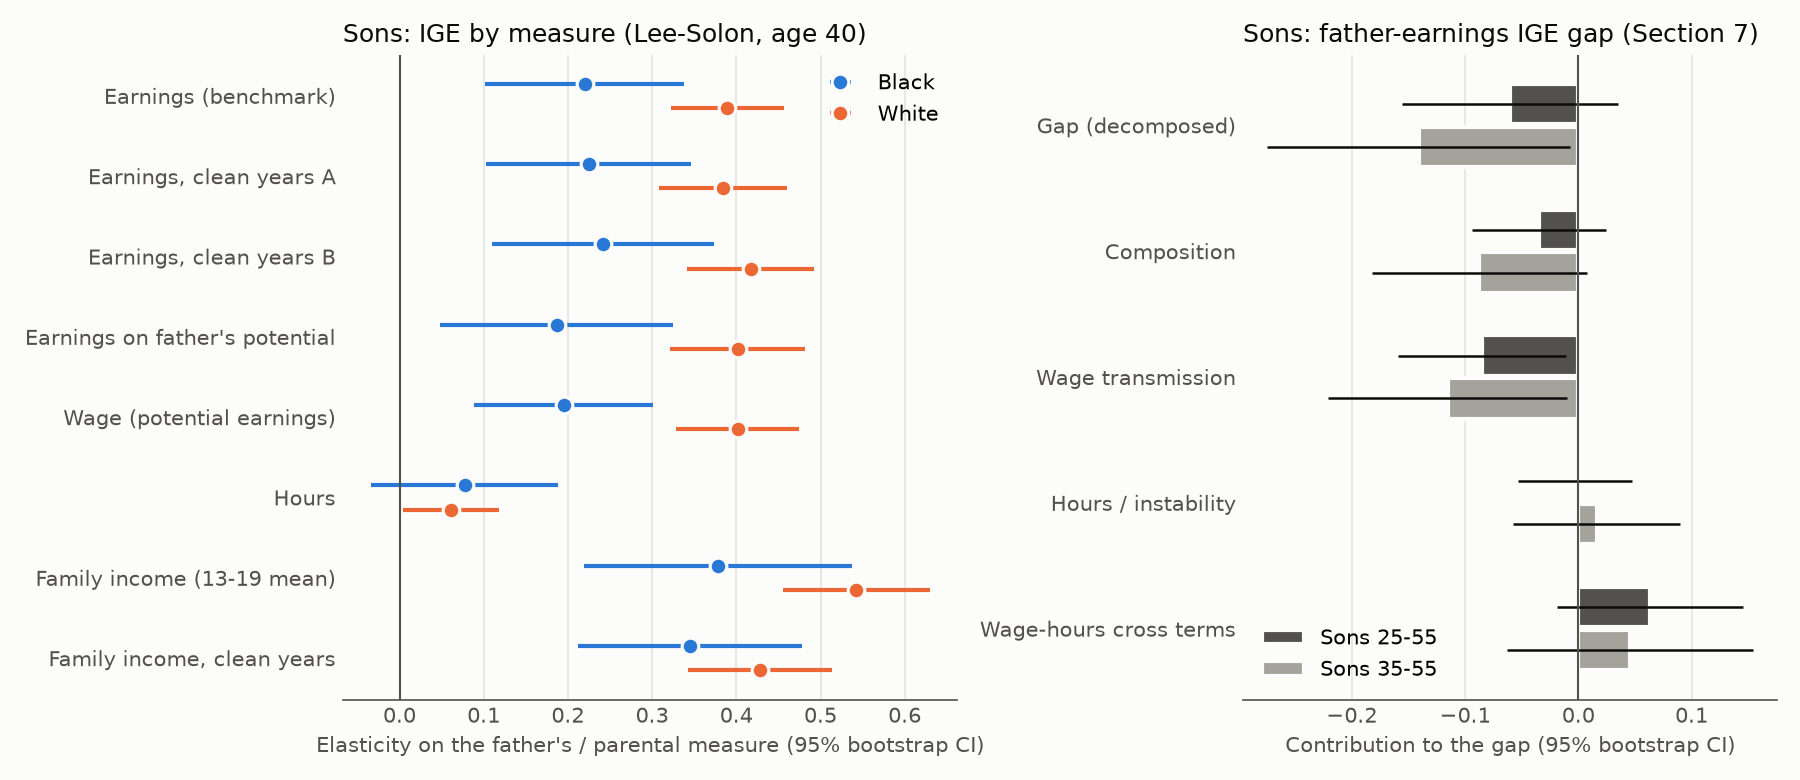
\includegraphics[width=\textwidth]{ige_decomposition.png}
\caption{What the IGE contains: elasticities by measure and the decomposition of the racial gap (PSID, sons)}
\label{fig:decomposition}
\begin{minipage}{\textwidth}\footnotesize \textit{Notes:} Left: elasticities of sons' outcomes with respect to the
father's (or parental) measure, Lee--Solon design at age 40, by race, with 95\% bootstrap confidence intervals; clean
years A exclude displacement and unemployment, B also reduced hours. Right: decomposition of the racial gap (plotted as Black $-$ White in this figure) in
the father-earnings IGE for sons 25--55 and 35--55 (Table~\ref{tab:decomposition}). This figure colours Black
estimates blue and White estimates orange. Code: \texttt{24.IGEDecomposition.py}.\end{minipage}
\end{figure}

\subsection{Designs that were not informative}

\paragraph{Lifetime means.} Averaging each son's earnings over his whole observed career averages the ages before
and after the divergence. In the lifetime-mean design the White--Black gap in the father-earnings IGE is 0.044
(0.050), against 0.169$^{**}$ (0.074) at age 40 in the age-interacted design.\footnote{\texttt{output/ige\_decomposition.md},
Sections 2 and 7. Code: \texttt{24.IGEDecomposition.py}.}

\paragraph{Father's working-life measure.} Measuring the father's earnings over his own working life (25--55) mixes
years after the son has left home; the gap is 0.129 (0.083). The childhood-window measure is the one the question
requires.

\paragraph{Re-weighting ratios and tercile slopes.} Ratios of re-weighted to raw gaps at one age are ratios of noisy
gaps (0.593, s.e.\ 0.653, for the family-income IGE), and IGE slopes within terciles of the parental distribution are
too noisy to be informative (0.802, s.e.\ 0.401, for Black sons in the top tercile). The band-by-band re-weighting and
the comparison below the median of Section~\ref{sec:ageprofile} use the whole profile and are the informative
versions.

\paragraph{Coded occupation changes.} Moves to higher-paying occupations coded from consecutive interviews fall with
parental income ($-0.031^{***}$), because PSID occupations are coded independently in each wave after 1980 and coded
changes contain much churning and coding noise. The level decomposition of Section~\ref{sec:careers} is used
instead.\footnote{\texttt{output/career\_wage\_growth.md}, Section 4. Code: \texttt{27.CareerWageGrowth.py}.}

\paragraph{A fast track inside well-paid cells.} The parental-income gradient of wage growth inside well-paid,
fast-growing cells (0.146$^{**}$) is larger than outside them (0.043), but the difference, 0.103 ($p=0.113$), is
imprecise.

\paragraph{Cleaning daughters' years.} Displacement and unemployment flags exist only for male heads in the PSID, so
daughters' own years cannot be purged of shocks.
